\documentclass[a4paper, 11pt, openright, twoside]{report}

\usepackage{graphicx}
\usepackage{polski}
\usepackage[english,polish]{babel}
\usepackage[utf8]{inputenc}
\usepackage[top=3.5cm,bottom=4.5cm,left=3.5cm,right=3.5cm, bindingoffset=0cm, footskip=2.5cm]{geometry}
\usepackage{setspace}
\usepackage{multirow}
\usepackage[unicode=true]{hyperref}
\usepackage{subcaption}
\usepackage{array}
\usepackage{amsmath}
\usepackage{placeins
}\usepackage[
    backend=biber,
    sorting=nty,
  ]{biblatex}
\usepackage{amssymb}
\usepackage{amsthm}
\usepackage{bm}
\usepackage{commath}
\usepackage{graphicx}
\usepackage{mathtools}
\usepackage{ragged2e}
\usepackage{tcolorbox}
\usepackage[normalem]{ulem}
\usepackage[absolute,overlay]{textpos}
\usepackage{xcolor}
\usepackage{algorithm}
\usepackage{algpseudocode}
\makeatletter
\renewcommand{\ALG@name}{Algorytm}
\renewcommand{\listalgorithmname}{List of \ALG@name s}
\makeatother
\addbibresource{export.bib}

\usepackage{xcolor}
\usepackage{listings}
\usepackage{caption}

\renewcommand\lstlistingname{listing}
\DeclareCaptionFont{forlst}{\footnotesize\scshape}
\captionsetup[lstlisting]{font=forlst}

\lstset{
language=C++,
basicstyle=\small\ttfamily,
keywordstyle=\color[rgb]{0.764,0.082,0.294},
commentstyle=\color[rgb]{0.278,0.553,0.560},
stringstyle=\color[rgb]{0.871,0.236,0.105},
breaklines=true,
showstringspaces=false,
columns=fixed,
keepspaces=true,
basewidth=0.5em
}

%\lstset{
%emph={if,else,for,return,do,break,while,const,static,public,struct},emphstyle=\color[rgb]{0,0.5,0},
%emph={[2]true, false},emphstyle={[2]\color[rgb]{0.266,0.184,0.949}}}

\lstset{
frame=topline,
belowcaptionskip=4pt,
framesep=8pt,
belowskip=12pt,
}


\DeclareCaptionFont{smallcap}{\small}
\captionsetup[figure]{font=smallcap}
\captionsetup[table]{font=smallcap}

\begin{document}

\begin{titlepage}

\begin{center}


\includegraphics[scale=1.25]{agh_nzw_s_pl_1w_wbr_pms}\\[0.2cm]
%
\includegraphics[scale=1.25]{agh_nzw_s_en_1w_wbr_pms}\\[0.2cm]

\textsc{Wydzial Informatyki, Elektroniki i Telekomunikacji}\\[0.2cm]

\textsc{Katedra Elektroniki}\\[1cm]

\textbf{Praca dyplomowa \\ inżynierska}\\[1cm]

{\huge \bfseries Automatyczna regulacja głośności z jednoczesnym tłumieniem tła akustycznego}\\[1cm]



\vfill

\begin{minipage}{0.8\textwidth}
\begin{flushleft}
{\large \emph{Imię i nazwisko:} \hfill Piotr \textsc{Radecki}}\\[0.1cm]
{\large \emph{Kierunek studiów:} \hfill \textsc{Elektronika i Telekomunikacja}}\\[0.1cm]
{\large \emph{Typ studiów:} \hfill \textsc{Stacjonarne}}\\[0.1cm]
{\large \emph{Opiekun pracy:} \hfill dr hab. inż. Konrad \textsc{Kowalczyk}, prof. AGH}\\[0.1cm]
\end{flushleft}
\end{minipage}\\[2cm]

Kraków 2021

\end{center}

\end{titlepage}


%\thispagestyle{empty}
\
\vfill

\begin{flushright}

\begin{minipage}{0.65\textwidth}

\textsc{Oświadczam, świadomy odpowiedzialności karnej za poświadczenie nieprawdy,  że niniejszą pracę dyplomową wykonałem osobiście i~samodzielnie i że nie korzystałem ze żródeł innych niż wymienione w pracy.}\\

\raggedleft \ \\[0.2cm]
\
\end{minipage}

\end{flushright}


\selectlanguage{polish}
\chapter*{Streszczenie}


W pracy inżynierskiej zaimplementowany został algorytm automatycznej kontroli głośności dla sygnałów mowy nagranych macierzą mikrofonową. Do zrealizowania użyto zaawansowanego algorytmu przetwarzania sygnałów jakim jest filtr LCMV. Otrzymany algorytm estymuje kierunki nadchodzenia dzwięku za pomocą algorytmu MUSIC i reguluje głośność pojedynczych mówców przy jednoczesnym tłumieniu zakłócenia jakim jest biały szum. Zaimplemntowane rozwiązanie bazuje na nagraniach z macierzy mikrofonowej. W ramach pracy stworzono również specjalny generator symulujący geometrię macierzy mikrofonej i pomieszczeń, w których rozchodzi się dzwięk. W celu zrealizowania pracy zapoznano się z fachową litaraturą naukową i napisano oprogramowanie w języku Python. Wykonana implementacja została poddana licznym testom. Sprawdzono wpływ czynników takich jak ilość źródeł i ich położenia, poziom szumu a także geometria pokoju i mikrofonu na jakość działania algorytmu. Uzyskane wyniki przeanalizowano i opisano. 

Praca ma następującą kompozycję: w rozdziale \ref{chapter-2} autor przedstawia teorię zagadnienia. W rozdziale \ref{chapter-3} przedstawione zostało rozwiązanie wraz z krótkim opisem użytych metod. W kolejnych rozdziałach znajdują się szczegóły implementacyjne (rozdział \ref{chapter-4}) i testy zaimplementowanego rozwiązania (rodział \ref{chapter-5}).

\newpage

\chapter*{Summary}

The goal of the thesis was to implement automatic gain control algorithm for speech signals recorded with microphone matrix. The project was accomplished using LCMV filter which is complex signal processing concept. The implemented method estimates directions of arrival of sound waves using MUSIC algorithm and adjusts loudness of users. Simultaneously it attenuates white noise. The solution is based on microphone array recordings. Author of this dissertation developed generator which simulates geometry of microphone array and room response. In order to write this thesis author conducted deep research including state-of-the-art scientific literature. The effect of this work is software solution written in Python programming language. The implementation was thoroughly tested. Influence of many factors including number of audio sources, signal to noise ratio and geometry of microphone array and room. Obtained results has been analysed and described. 

Structure of the paper is as follows. In chapter \ref{chapter-2} author has shortly described theory of the problem. In chapter \ref{chapter-3} the solution was presented along with short description of used methods. Chapter \ref{chapter-4} contains details regarding implementation. Finally chapter \ref{chapter-5} presents tests of the system.

\selectlanguage{polish}
%\selectlanguage{english}

\tableofcontents
\addcontentsline{toc}{chapter}{Spis treści}

\chapter{Wstęp}
\section{Wprowadzenie}

Algorytmy automatycznej kontroli głośności(AGC) są ważnym elementem współczesnych systemów przetwarzania sygnałów audio. Zarówno do zastosowań telekomunikacyjnych, konferencyjnych jak i obróbki nagrań. Takie algorytmy mają na celu zapewnić stały poziom głośności mówców zarówno w czasie jak i między sobą.
Ważne jest aby takie algorytmy skutkowały wysokim poziomem sygnału do szumu(SNR) jak i wysokim stosunkiem sygnału do szumu do pozostałych interferencji- na przykład pogłosu.

Najprostszym rozwiązaniem jest zastosowanie prostego systemu jednokanałowego[JAKAŚ REFKA!]. W takim systemie możlie jest tylko sterowanie głośnością sygnału wejściowego, na podstawie chwilowej wartości obwiedni. Uniemożliwia on jednak różny poziom wzmocnienia dla różnych mówców i usunięcie interferencji.

Rozwiązaniem bardziej skomplikowanym, zarówno od strony sprzętowej, programistycznej i czasu obliczeń jest użycie systemu z wieloma mikrofonami. Taki system umożliwia pożądane rozróżnienie między mówcami i eliminację interferencji[REFKA!]. W systemie takim możliwa jest estymacja wektora sterującego, czyli kierunków nadchodzenia fali, a co za tym idzie mocy nadchodzącej z wybranych stron i zastosowanie odpowiednich filtrów, które wzmacniają sygnał z żądanych kierunków.

W tej pracy skupiono się właśnie na drugim z wymienionych rodzajów algorytmów AGC. W pracy zostanie przedstawiona praktyczna implementacja bazująca na nagraniach z macierzy mikrofonowych.

\begin{figure}[h]
    \centering
    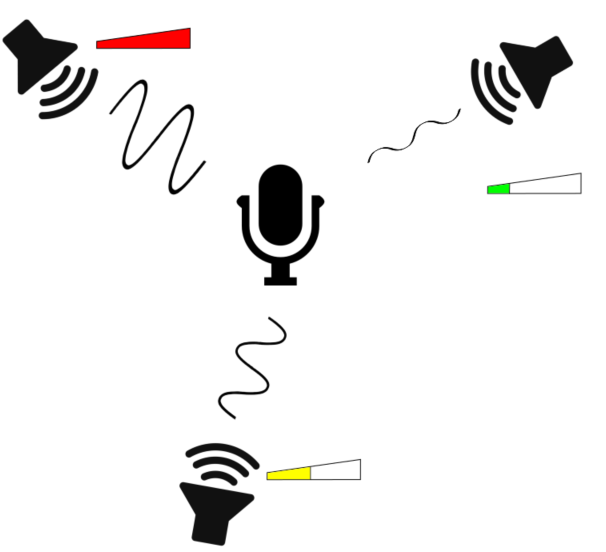
\includegraphics[width=\textwidth]{Images/setup.png}
    \caption{Graficzna reprezentacja problemu}
    \label{fig:setup}
\end{figure}

\section{Cel}
Celem pracy inżynierskiej była praktyczna implementacja istniejącego algorytmu AGC z tłumieniem tła akustycznego, wraz z estymacją kierunku nadchodzenia fali. Wybrany algorytm spełnia cechy wymienione w poprzedniej sekcji,tj. pozwala na regulację głośności nagrania zarówno w czasie jak i między mówcami i minimalizację zakłóceń. Jako zakłócenie do eliminacji przyjęto w niniejszej pracy biały szum gaussowski.

\section{Zakres wykonanej pracy}
Pierwszym z etapów pracy inżynierskiej było zapoznanie się autora pracy z dostępnymi publikacjami opisującymi zarówno tematykę AGC jak i generalną tematykę przetwarzania sygnałów dla macierzy czujników i wybór metody. 
Kolejnym etapem pracy. Następnie dokonany wyboru środowiska pracy- był to język Python. Szczegółowy opis użytych narzędzie znajduje się w [blablka]. Następnie autor pracy napisał symulator umożliwiający generację sygnałów mikrofonowych. Dalsza część realizacji pracy obejmowała- zaplanowanie praktycznej implementacji systemu, wykonanie tej implementacji i testy przy użyciu symulatora[tu wszędzie jaka sekcja itp].



\chapter{Analiza Teoretyczna problemu}
\label{chapter-2}
\section{Model systemu}

Z uwagi na to, że litera "x" jest wielokrotnie używana w opisie modelu autor pracy zdecydował się na wstępie wprowadzić krótką legendę używanych oznaczeń z tą literą:
\begin{itemize}
    \item $x$ pisane czcionką typu $italic$ oznacza współrzędną w układzie kartezjańskim
    \item $\mathrm{x(t)}$ lub $\mathrm{x(n)}$ oznaczają sygnał w dziedzinie czasu (ciągłej lub dyskretnej)
    \item $\mathrm{X}(f)$, $\mathrm{X(k)}$ lub $\mathrm{X(k,n)}$ oznacza reprezentację tego samego sygnału w dziedzinie częstotliwości
    \item $\bm{\mathrm{x}}(f)$, $\bm{\mathrm{x}}(k)$ lub $\bm{\mathrm{x}}(k,n)$ pisane pogrubioną czcionką oznacza wektor o długości $M$ reprezentujący sygnał na $M$ mikrofonach w dziedzinie częstotliwości.
\end{itemize}


\noindent Na wstępie postanawia się intujcyjnie przedstawić pochodzenie wzorów użytych poniżej. W szczególności interesujący jest wektor sterujący $\bm{\mathrm{a}}$.

\noindent Zakłada się, że źródła znajdują się w sferze dalekiej, tj. odległość źródła od mikrofonu jest znacznie większa od długości fali i fizycznych wymiarów mikrofonu. Co więcej zakłada się, że mikrofony są na tyle blisko siebie, że nie występuje pomiędzy nimi tłumienie.

\noindent Na mikrofon pada sygał nadchodzący z kierunku $\theta_{l}$.
Zapis sygnału w punkcie $\bm{\mathrm{d}}_{0} = [0,0]$ to $\mathrm{x}_{l}(t,\bm{\mathrm{d}}_{0})$. Opóźnienie w czasie tego sygnału na mikrofonie położonym w $\bm{\mathrm{d}}_{\mathrm{m}} = [x_{\mathrm{m}},y_{\mathrm{m}}]$ względem punktu $\bm{\mathrm{d}}_{0}$ wynosić będzie zatem pewne $\tau$. Różnica dróg między punktami wyniesie $\Delta d$ tak jak na rysunku \ref{fig:direction}. Za pomocą prostej trygonometrii może zostać udodnione, że:
\begin{equation}
    \label{equation:2.4}
    \Delta d = -x_{\mathrm{m}}\cos{\theta_{l}} - y_{\mathrm{m}}\sin{\theta_{l}}
\end{equation}
Następnie przyjmując prędkość rozchodzenia się fali w ośrodku $c$ można zapisać, że:
\begin{equation}
    \label{equation:2.5}
    \tau = \dfrac{\Delta d}{c}
\end{equation}

\noindent Przechodząc z sygnałem do dziedziny częstotliwości i zakładając parę transformat Fouriera $\mathrm{x}_{l}(t,\bm{\mathrm{d}}_{0})\xleftrightarrow{}\mathrm{X}_{l}(f,\bm{\mathrm{d}}_{0})$ można zapisać, że:
\begin{equation}
    \label{equation:2.6}
    \mathrm{x}_{l}(t,\bm{\mathrm{d}}_{\mathrm{m}}) \xleftrightarrow{} \mathrm{X}_{l}(f,\bm{\mathrm{d}}_{0})e^{j 2 \pi f \tau} =
    \mathrm{a}_{l}(f,\bm{\mathrm{d}}_{\mathrm{m}}) \mathrm{X}_{l}(f,\bm{\mathrm{d}}_{0}) 
\end{equation}

\noindent W przypadku wielu mikrofonów ustawionych na pozycjach $\{\bm{\mathrm{d}}_{1}...\bm{\mathrm{d}}_{M} \}$:
\begin{equation}
    \label{equation:2.7}
    \bm{\mathrm{x}}_l(f)=
    \bm{\mathrm{a}}_l(f)\mathrm{X}_{l}(f,\bm{\mathrm{d}}_{0})
\end{equation}

\noindent Gdzie wektor sterujący $\bm{\mathrm{a}}_{l} = [\mathrm{a}_{l}(\bm{\mathrm{d}}_{1})...\mathrm{a}_{l}(\bm{\mathrm{d}}_{M})]$.Taki zapis równania może być przeniesiony do dziedziny krótkoczasowej transformaty Fouriera(ang. STFT). Wówczas otrzymane zostanie równanie \ref{equation:2.3}

\begin{figure}[h]
    \centering
    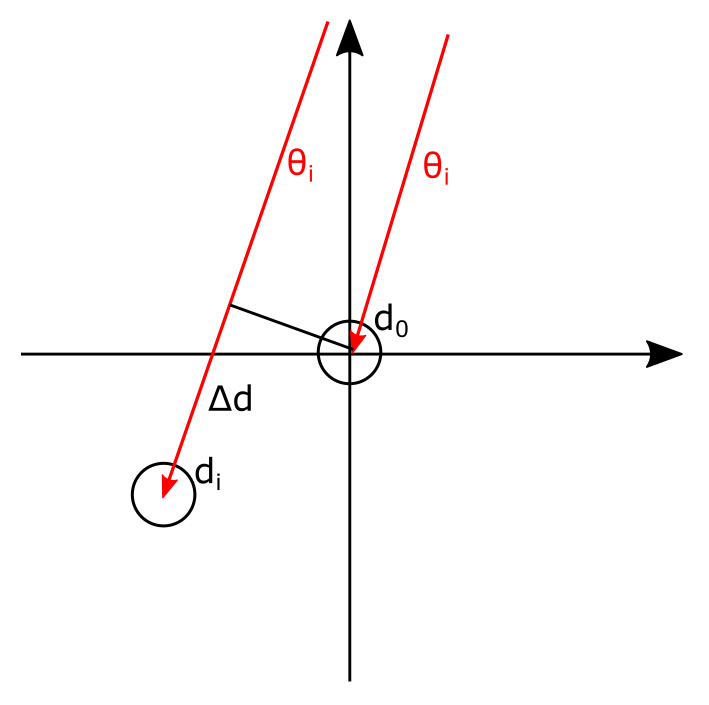
\includegraphics[width=\textwidth]{Images/direction.png}
    \caption{Opóźnienie fali na mikrofonie}
    \label{fig:direction}
\end{figure}

\newpage 

Poniższy model sygnału jest zaczerpnięty z \cite{Thiergart2013} i \cite{Braun2014}, z tą różnicą, że w tej pracy wszystkie zakłócenia traktowane są razem.

\noindent Zakłada się, że używanym czujnikiem jest macierz $M$ mikrofonów dookólnych rozłożonych na płaskiej powierzchnii w pozycjach $\{\bm{\mathrm{d}}_1...\bm{\mathrm{d}}_M\}$.

\noindent Na czujnik pada $L$ fal płaskich, gdzie $M > L$ ośrodku izotropowym i jednorodnym, w którym obecne są zakłócenia.Każda z fal nadbiega z kąta $\{{\theta}_1...{\theta}_L\}$ Model może być zapisany w dziedzinie STFT jako:
\begin{equation}
    \label{equation:2.1}
    \bm{\mathrm{x}}(k,n)
    =
    [\mathrm{X}(k,n,\bm{\mathrm{d}}_{1})
    ...
    \mathrm{X}(k,n,\bm{\mathrm{d}}_{M})]^{T}
\end{equation}
lub alternatywnie jako:
\begin{equation}
    \label{equation:2.2}
    \bm{\mathrm{x}}(k,n)=
    \sum_{l=1}^{L} \bm{\mathrm{x}}_{l}(k,n)
    + \bm{\mathrm{x}}_{\mathrm{n}}(k,n)
\end{equation}

\noindent gdzie $\bm{\mathrm{x}}_l(k,n)$ to wektor natężeń l-tej fali na poszczególnych mikrofonach a $\bm{\mathrm{x}}_{\mathrm{n}}(k,n)$ to wektor natężenia tła akustycznego na mikrofonach.
Oznacza to, że otrzymany na każdym z mikrofonów sygnał jest mieszaniną sygnału z kilku różnych źródeł i zakłóceń.

\begin{figure}[h]
    \centering
    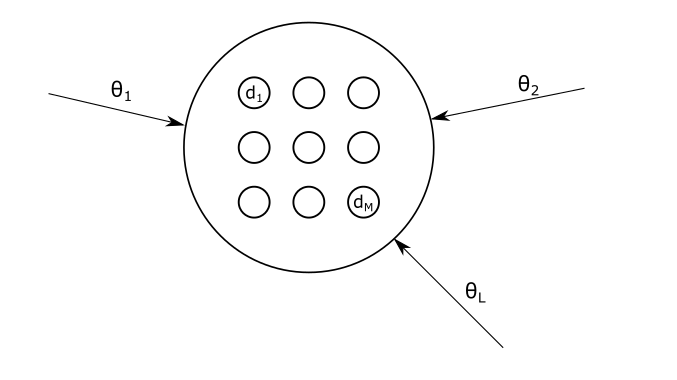
\includegraphics[width=\textwidth]{Images/model.png}
    \caption{Model systemu}
    \label{fig:model}
\end{figure}


\noindent Każdy z wektorów $\bm{\mathrm{x}}_l(k,n)$ może być opisany za pomocą równania:
\begin{equation}
    \label{equation:2.3}
    \bm{\mathrm{x}}_l(k,n)=
    \bm{\mathrm{a}}_l(k,n)X_{l}(k,n,\bm{\mathrm{d}}_{0})
\end{equation}
\noindent gdzie $\bm{\mathrm{a}}_l(k,n)X_{l}(k,n,\bm{\mathrm{d}}_{0})$ jest wartością natężenia l-tej fali w punkcie referencyjnym $\bm{\mathrm{d}}_0$. Często w publikacjach, na przykład w \cite{Braun2014} za punkt referencyjny jest wybierane położenie mikrofonu $\bm{\mathrm{d}}_1$. Autor pracy zdecydował się jednak na bardzej ogólne podejście do problemu.

\noindent W pracy zakłada się, że kierunek nadchodzenia fali nie jest znany ale znana jest ilość źródeł L w systemie.


\newpage
\section{Postawiony Problem}

W wyżej opisanym modelu mogą zostać zdefiniowane następujące potencjalne problemy:
\begin{itemize}
    \item Sygnał $\bm{\mathrm{x}}_{i}$ może charakteryzować się amplitudą różną od sygnału $\bm{\mathrm{x}}_{j}$ co będzie skutkować zagłuszaniem jednego z użytkowników systemu przez innego 
    \item Natężenie sygnału $\bm{\mathrm{x}}_{i}$ może mocno fluktować w czasie z uwagi na przykład na przybliżanie i oddalanie się mówcy od mikrofonów
    \item W systemie występuje tło akustyczne- niechciane zakłócenia, których wyeliminowanie jest pożądanym działaniem.
\end{itemize}

\chapter{Rozwiązanie problemu}
\label{chapter-3}

\section{Model rozwiązania}

W pracy zdecydowano się rozwiązać problem na bazie metody opisanej w publikacji \cite{Braun2014}. W tej sekcji zostanie podany zbiór metod użytych do rozwiązanie problemu. Zdefiniowanie i opis poszczególnych metod nastąpi w kolejnych sekcjach rozdziału.

\noindent Przetwarzanie sygnału zaczyna się od obliczenia STFT nagrania wejściowego. Następnie odbywa się przetwarzanie przedstawione na \ref{fig:block_diagram}. Na początku obliczona zostaje macierz widmowej gęstości mocy sygnału (PSD). Następnie za jej pomocą estymowany jest kierunek nadchodzenia fal (DOA). Dzięki połączeniu tych wartości możliwe jest zastosowanie algorytmu automatycznej regulacji głośności (AGC). Ostatnim krokiem jest zastosowanie filtru LCMV, który jako argumenty przyjmuje żądane poziomy wzmocnień, wyestymowane kierunki i sygnał wejściowy. Taki filtr produkuje sygnał wyjściowy. 

\begin{figure}[h]
    \centering
    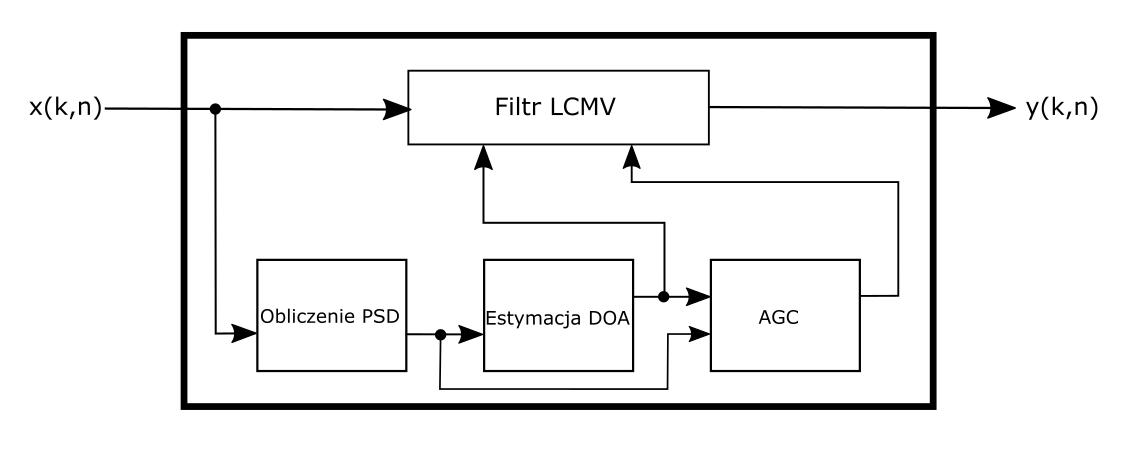
\includegraphics[width=\textwidth]{Images/block_diagram.png}
    \caption{Diagram blokowy}
    \label{fig:block_diagram}
\end{figure}

\section{Widmowa gęstość mocy}

Widmowa gęstość mocy może być zapisana jako:
\begin{equation}
    \label{equation:PSD}
    \phi_{l}(k,n) = \mathrm{E}
    \{|X_{l}(k,n,\bm{\mathrm{d}}_{0})|\}
\end{equation}
Macierz widmowej gęstości mocy definiuje się następująco:

\begin{equation}
    \label{equation:PSD matrix}
    \mathrm{\Phi}(k,n) = \mathrm{E} \, \{\bm{\mathrm{x}}(k,n) \bm{\mathrm{x}}^{H}(k,n)\}
\end{equation}

W praktyce jest obliczana jako średnia z $N$ zebranych próbek:
\begin{equation}
    \label{equation: PSD in practice}
    \mathrm{\Phi}(k,n)=
    \dfrac{1}{N} \sum_{i = n-N}^{n-1}
    \bm{\mathrm{x}}(k,i) \bm{\mathrm{x}}^{H}(k,i)
\end{equation}

Zgodnie z \cite{Thiergart2013}, zakładając, że wszystkie elementy równania \ref{equation:2.2} są nieskorelowane, można zapisać:

\begin{equation}
    \label{equation:PSD signal noise}
    \bm{\mathrm{\Phi}}(k,n) = 
    \sum_{l=1}^{L} \bm{\mathrm{\Phi}}_{l}(k,n) +
    \bm{\mathrm{\Phi}}_{\mathrm{n}}(k,n)
\end{equation}

Gdzie odpowiednio $\bm{\mathrm{\Phi}}_{l}(k,n)$ i $\bm{\mathrm{\Phi}}_{\mathrm{n}}(k,n)$ są macierzami PSD odpowiednio $l$-tej padającej fali i zakłóceń.

\section{Przestrzenna funkcja głośności}

Ważnym elementem systemu będzie sterowanie tak zwaną przestrzenną funkcją głośnośni $G(\theta_{l},n)$. Funkcja ta jest odpowiedzialna za utrzymywanie głośności sygnału wyjściowego na założonym poziomie:

\begin{equation}
    \label{equation:G}
    \mathrm{Y}(k,n)= 
    \sum_{l=1}^{L} G(\theta_{l},n)
    \mathrm{X}_{l}(k,n,\bm{\mathrm{d}}_0)
\end{equation}

\section{Filtr LCMV}

Punktem wyjściowym dla definicji filtru LCMV jest próba zapisania estymaty sygnału wyjściowego $\hat{\mathrm{Y}}(k,n)$ jako:
\begin{equation}
    \label{equation:Y estimation}
    \hat{\mathrm{Y}}(k,n)=
    \bm{\mathrm{w}}^{\mathrm{H}}(k,n)
    \bm{\mathrm{x}}(k,n)
\end{equation}

\noindent Aby znaleźć współncyznniki filtru $\bm{\mathrm{w}}_{\mathrm{n}}(k,n)$, które pozwolą jak najlepiej przybliżyć żądane rozwiązanie należy rozwiązać problem optymalizacyjny zdefiniowany przez dwa poniższe równania:
\begin{equation}
    \label{equation:argmin}
    \bm{\mathrm{w}}_{\mathrm{n}}(k,n) = 
    \underset{\bm{\mathrm{w}}}{\mathrm{arg \, min}} \,
    \bm{\mathrm{w}}^{\mathrm{H}}
    \bm{\mathrm{\Phi}}_{n}
    \bm{\mathrm{w}}
\end{equation}

\begin{equation}
    \label{equation:constraint}
    \bm{\mathrm{w}}^{\mathrm{H}}
    \bm{\mathrm{a}}_{l}(k,n)=
    G(\theta_{l},n),
    \, \, l \in \{1,2,...,L\}
\end{equation}

Ten zapis oznacza, że żądany filtr powinien minimalizować podawane na wejście zakłócenia \ref{equation:argmin} i odpowiednio sterować głośnościami poszczególnych nadchodzących fal \ref{equation:constraint}. Rozwiązanie tak postawionego problemu można znaleźć w \cite{Thiergart2013} zaś wyprowadzenie w \cite{Frost1972}:

\begin{equation}
    \label{equation:lcmv formula}
    \bm{\mathrm{w}}_{\mathrm{n}}=
    \bm{\mathrm{\Phi}}_{n}^{-1}\bm{\mathrm{A}}
    [\bm{\mathrm{A}}^{\mathrm{H}} \bm{\mathrm{\Phi}}_{n} \bm{\mathrm{A}}]^{-1}
    \bm{\mathrm{g}}
\end{equation}

\noindent Gdzie macierz $\bm{\mathrm{A}}(k,n)=
[\bm{\mathrm{a}}_{1}...\bm{\mathrm{a}}_{L}]$ zaś wektor $\bm{\mathrm{g}}(n)=[G(\theta_{1},n)...G(\theta_{L},n)]^{T}$.

\section{Algorytm MUSIC}

MUSIC(ang. Multiple Emitter Location and Signal Parameter Estimation) został opisane w \cite{Schmidt1986}. Nowocześniejsze opracowania można też znaleźć w \cite{DOA} i \cite{Benesty2008} Algorytm pozwala wyestymować kierunki nadchodzenia fali w systemie zawierającym wiele źródeł. Algorytm zakłada przyjęty model sygnału z założeniem, że tło akustyczne to wyłącznie biały szum gaussowski. Obecność innych zakłóceń pogarsza działanie systemu.

\noindent Na potrzeby tej pracy zostanie przedstawiony skrótowo algorytm. Wyprowadzenie znajduje się w wyżej cytowanej publikacji. 
Definiuje się zapis $\bm{\mathrm{a}}(k,n,\theta)$, oznaczający wektor sterującym dla kąta padania $\theta$ i indeksu czasowo-częstotliwościowego $(k,n)$ oraz $\bm{\mathrm{\Phi}}(k,n)$ oznaczający macierz PSD sygnału dla tego samego indeksu czasowo-częstotliwościo

\noindent Liczba nadchodzących fal $L$ może być wyestymowana na przykład zgodnie z publikacją \cite{n_src}. W tej pracy zakłada się jednak, że liczba źródeł jest znana.

\noindent W rozkładzie na wartości własne macierzy $\bm{\mathrm{\Phi}}(k,n)$ wektory własne powiązane z L największymi wartościami własnymi nazywa się wektorami podprzestrzenii sygnału i oznacza jako $\bm{\mathrm{s}}_{i}$, zaś pozostałe wektory- wektorami z podprzestrzenii szumu $\bm{\mathrm{e}}_{i}$. Macierz $\bm{\mathrm{E}}(k,n)$ zawiera w kolejnych kolumnach kolejne wektory podprzestrzenii szumu.

\begin{equation}
    \label{equation:eigenvectors}
    \bm{\mathrm{E}}(k,n)=
    [\bm{\mathrm{e}}_{1}(k,n)...
    \bm{\mathrm{e}}_{M-L}(k,n)]
\end{equation}

\noindent Następnie definiuje się funkcję:
\begin{equation}
    \label{equation:P}
    P(\theta,k,n)=
    \dfrac{1}{
    \bm{\mathrm{a}}^{\mathrm{H}}(\theta,k,n)
    \bm{\mathrm{E}}(k,n)
    \bm{\mathrm{E}}^{\mathrm{H}}(k,n)
    \bm{\mathrm{a}}(\theta,k,n)
    }
\end{equation}
\noindent 
$L$ największych maksimów lokalnych takiej funkcji w dziedzinie kątów uznaje się za wyestymowane kierunki nadchodzenia fali.

\noindent Celem algorytmu jest jednak uzyskanie jednego kierunku nadchodzenia fali dla $n$-tej chwili czasowej. Propozycją autora pracy jest zdefiniować taką funkcję $P_{a}(\theta,n)$, że:
\begin{equation}
    \label{equation:Pa}
    P_{a}(\theta,n) = 
    \dfrac{1}{K}\sum_{k=1}^{K}\,P(\theta,k,n)   
\end{equation}

\noindent Ponownie, $L$ największych maksimów lokalnych wskazuje kierunki nadchodzenia fali.

\newpage
\section{Automatyczna regulacja głośności}

Autor publikacji \cite{Braun2014} proponuje zdefiniowanie funkcji przestrzennego rozkładu głośności(ang. SLD) zapisanego jako:

\begin{equation}
    \label{equation:SLD}
    \Psi(\theta,n)=
    \sum_{k=1}^{K} \beta^{2}(k)
    \sum_{l=1}^{L}\delta_{\theta,\theta_{l}}
    \, \phi_{l}(k,n)
\end{equation}

\noindent Gdzie $(k,n)$ to indeksy czasowo częstotliwościowe, $\delta_{\theta,\theta_{l}}$ to delta Kroneckera- sygnał przyjmujący wartość $1$ dla $\theta_{l}$ i $0$ dla pozostałych.

\noindent Aby wyestymować PSD $\phi_{i}$ $i$-tej fali dokonuje się filtracji filtrem LCMV takim, że:
\begin{equation}
    \label{equation:power estimation}
    \bm{\mathrm{w}}^{\mathrm{H}}\bm{\mathrm{a}}_{l}(k,n)=
    \begin{cases}
        1 \quad l=i \\
        0 \quad l \neq i
    \end{cases}
\end{equation}


\noindent Wartość współczynników $\beta$ może być określona na podstawie istniejących norm, na przykład \cite{coef}. Autor tej pracy iżynierskiej zdecydował jednak przyjąć wartość:

\begin{equation}
    \label{equation:beta}
    \beta(k) = 1, \,\,\,\ k=\{1,2,...,K\}
\end{equation}

\noindent Definiuje się także długoczasową funkcję przestrzennego rozkładu głośności zdefiniowaną jako:

\begin{equation}
    \label{equation:LT_SLD}
    \Psi(\theta,n)=
    \alpha_{LT}\Psi_{LT}(\theta,n-1)
    +(1-\alpha_{LT})\Psi(\theta,n)
\end{equation}

\noindent To działanie ma na celu wygładzenie funkcji w dziedzinie czasu. Głośność sygnału powinna być niewrażliwa na fluktuacje o bardzo dużych częstotliwościach. Taka definicja funkcji jest tożsama z filtracją dolnoprzepustową za pomocą filtra o nieskończonej odpowiedzi impulsowej(IIR).

\noindent Funkcje nie są zależne od składowej częstotliwościowej bo celem pracy jest wzmocnienie amplitudy całego sygnału a nie poszczególnych pasm.

\noindent Przestrzenną funkcje głośności dla danego kąta możnaby otrzymać za pomocą:

\begin{equation}
    \label{equation:sqrt}
    G(\theta,n)=
    \sqrt{\dfrac{\Psi_{target}(\theta)}{
    \Psi_{LT}(\theta,n)}}
\end{equation}

\noindent Należy jednak zauważyć, że tak obliczona funkcja prowadziłaby do silnego wzmocnienia kierunków, w których nie ma sygnału. Co za tym idzie wzmacniane byłoby tłoakustyczne. Kilkustopniowy błąd estymacji kierunku nadchodzenia fali mógłby w praktyce uniemożliwić poprawne działanie systemu. Aby to uniemożliwić definiuje się minimalną moc uznawaną za sygnał $\Psi_{min}(n)$. Obliczona może być jako:

\begin{equation}
    \Psi_{\min}(n)=
    \max({\dfrac{1}{2\pi} \int_{0}^{2\pi} \Psi(\theta,n) \, \mathrm{d}\theta, \, \Psi_{0}})
\end{equation}
Gdzie $\Psi_{0}$ jest pewną ustaloną granicą.

\newpage

\noindent Następnie  dany jest algorytm do obliczenia wygładzonej przestrzennej funkcji głośności $G'(\theta,n)$:


\begin{algorithm}
  \label{alg:gprim}
  \caption{Obliczanie $G'(\theta,n)$}
  \begin{algorithmic}[1]
    \State Zainicjalizuj $G'(\theta,n)$ wartością 1 dla każdego kierunku
    
    \State  Znajdź maksimum globalne funkcji LT-SLD w dziedzinie kąta($\theta_{\max}$) i oblicz przestrzenną funkcją głośności $G(\theta_{max},n)$ za pomocą
    
    \State Wygeneruj okno przestrzenne o określonej szerokości $\Theta$, które ma wzmocnienie $1$ na brzegach i $G(\theta_{max},n)$ w środku.
    
    \State Umieść okno w $\theta_{\max}$ i wyzeruj wartości funkcji LT-SLD w punktach pokrytych przez okno.
    
    \State Kontynnuj krok 2 tak długo aż wszystie punkty funkcji LT-SLFD są poniżej progu $\Psi_{\min}$.
  \end{algorithmic}
\end{algorithm}

\noindent Następnie oblicza się funkcję wygładzającą $\widehat{G}(\theta,n)$:

\begin{equation}
    \label{equation:Ghat}
    \widehat{G}(\theta,n)=
    \alpha_{G}\widehat{G}(\theta,n)
    + (1-\alpha_{G})G'(\theta,n)
\end{equation}


\noindent Funkcja tej operacji jest taka sama jak \ref{equation:LT_SLD}. Otrzymane $\widehat{G}$ wstawia się do równania \ref{equation:constraint}.







\chapter{Szczegóły Implementacyjne}
\label{chapter-4}

\section{Użyte narzędzia}

\noindent Projekt inżynierski został napisany zaimplementowany jako program komputerowy w języku python. Do realizacji zostały użyte głównie paczki:

\begin{itemize}
    \item numpy- paczka służąca do obliczeń naukowych. Udostępnia rozbudowane API do algebry liniowej i przetwarzania sygnałów.
    \item scipy- moduł umożliwiający obliczenia matematyczne i techniczne, w szczególności przetwarzanie sygnałów stosowane w tej pracy
    \item matplotlib- paczka służąca do wizualizacji danych.
    \item rir generator- moduł umożliwiający symulację odpowiedzi impulsowej pokoju
\end{itemize}

\noindent Więcej informacji można znaleźć w dokumentacji paczek \cite{numpy}, \cite{matplotlib}, \cite{rir} i \cite{scipy}.

\section{Metologia rozwoju programu}

\noindent Realizacja pracy była podzielona na stworzenie właściwego programu opisane szczegółowo w rodziale \ref{chapter-3} i na stworzenie generatora symulującego rzeczywisty sygnał mikrofonowy z dodatkiem zakłóceń.


W założeniach oprogramowanie miał mieć charakter obiektowy. Główne bloki zostały zaimplementowane jako klasy, które komunikują się między sobą za pomocą interfejsów. Takie rozwiązanie powoduje usystematyzowaną strukturę projektu i umożliwia łatwy rozwój oprogramowania w przyszłości. Przykładem jest implementacja algorytmu MUSIC. Klasa MUSIC dziedziczy po klasie abstrakcyjnej DOA. W ten sposób proste w przyszłości będzie dopisanie w programie innego algorytmu estymacji kierunku nadchodzenia fali jako innej klasy dziedziczącej po DOA. Poniżej przedstawiono diagram klas w konwencji UML \cite{uml}:

\begin{figure}[h!]
    \centering
    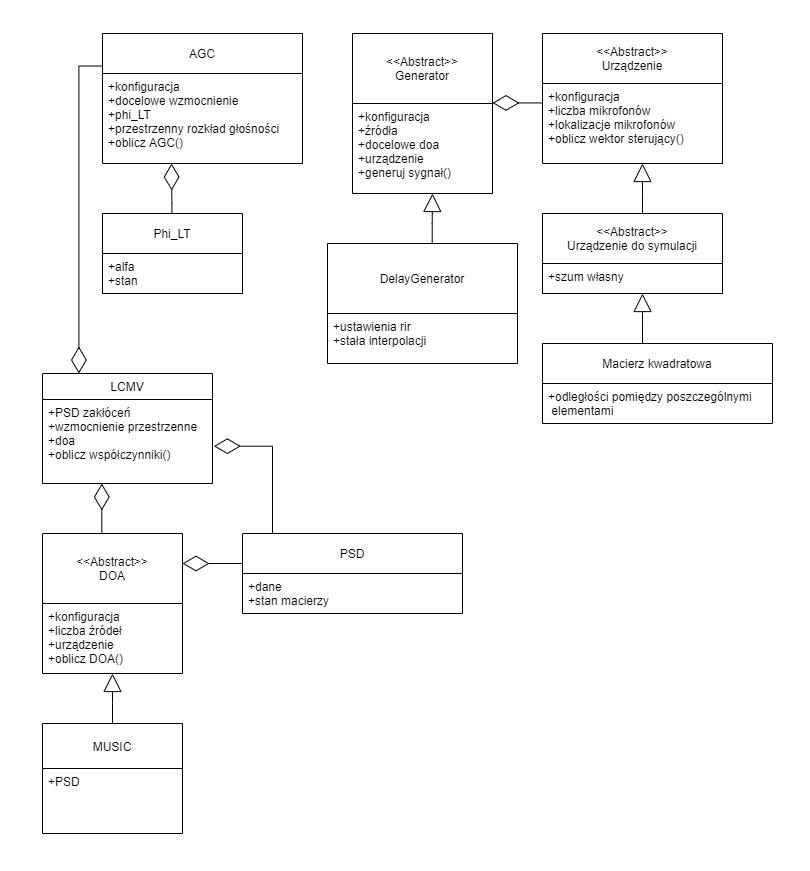
\includegraphics[width=\textwidth]{Images/uml_pl.png}
    \caption{Diagram klas}
    \label{fig:classes}
\end{figure}


\noindent W diagramie \ref{fig:classes} skrótowo opisano klasy. Nazwy nie odpowiadają( poza DelayGenerator) nazwom w kodzie. Nie są również dodane wszystkie składowe i metody. Schemat ma za zadanie przedstawić koncepcyjnie zaimplementowane rozwiązanie i pokazać podejście autora pracy do implementacji systemu.


\newpage

\section{Generator}

Generator pełni ważną rolę w projekcie inżynierskim. Z tego powodu postanawia się poświęcić mu osobną sekcję w tekście. 

\noindent Generator przyjmuje jako wejścia następujący dane:

\begin{itemize}
    \item Obiekt macierzy mikrofonowej
    \item Sygnały dzwiękowe 
    \item Funkcję kąta w czasie
    \item Funkcję wzmocnienia w czasie
    \item Opcjonalnie informacje o geometrii pokoju i o tym czy symulacja pogłosu jest włączona
\end{itemize}

\noindent Schemat działania generatora jest względnie prosty. Przyjmuje się model przedstawiony w rozdziale \ref{chapter-2}. Zakłada się, że sygnał wejściowy odpowiada wartości sygnału w punkcie $\bm{\mathrm{d}}_{0}$. Posiłkując się równaniami \eqref{equation:2.4} i \eqref{equation:2.5} można zapisać, że:

\begin{equation}
    \label{equation:delay model}
    \mathrm{x}_{l}(\bm{\mathrm{d}}_{m},t) = 
    \mathrm{x}_{l}(\bm{\mathrm{d}}_{0},t-\tau)
\end{equation}

\noindent Gdzie $\mathrm{x}_{l}(\bm{\mathrm{d}}_{m},t)$ to wymuszenie $l$-tej fali dzwiękowej w punkcie $\bm{\mathrm{d}}_{m}$. W takim układzie możliwe są bieżące zmiany opóźnienia bazując na pozycji źródła. Dodatkowo możliwa jest generacja białego szumu $n(t)$. Biały szum o mocy $\sigma$ może być przedstawiony jako zmienna losowa z rozkładu gaussowskiego o średniej 0 i wariancji $\sigma$.

\noindent Generator umożliwia symulację pomieszczenia, w  którym znajduje się mikrofon. Za pomocą paczki rir generator \cite{rir} generowana jest odpowiedź impulsowa pokoju $\bm{\mathrm{h}}(t)$. Tak generowana odpowiedź nazywana będzie później pogłosem. Szczegóły dotyczące genezy takiego sposoby symulacji pomieszczenia mogą być znalezione w książce \cite{Kuttruff}. Ostatecznie zatem sygnał wejściowy na $m$-tym mikrofonie może być zapisany w dziedzinie czasu jako:

\begin{equation}
    \label{equation:full generator}
    \mathrm{x}(t,\bm{\mathrm{d}}_{m})=
    \sum_{l=1}^{L}
    \mathrm{x}_{l}(\bm{\mathrm{d}}_{0},t-\tau_{l,m})*
    h_{l}(t)+ n(t)
\end{equation}

\noindent Z uwagi na to, że w celu generacji filtra pogłosowego konieczne są konkretne pozycje źródeł i mikrofonu, włączenie symulacji pomieszczenia nie pozwala na zmiany pozycji źródeł w czasie symulacji.




\section{Schemat przetwarzania danych}

Algorytm przetwarza nagrane pliki dzwiękowe. Składa się z następujących kroków:

\begin{algorithm}
  
  \caption{Schemat przetwarzania}
  \begin{algorithmic}[1]
    \State Na wejście trafia M ścieżek dzwiękowych
    
    \State Sygnał jest przetwarzany do reprezentacji STFT
    
    \State Przetwarzanie odbywa się w pętli po kolejnych indeksach czasowych, nazywanych ramkami
    
    \State Na wyjściu przetwarzania sygnałów zwracany jest sygnał $Y(k,n)$ jako STFT
    
    \State Dane wyjściowe są przetwarzane za pomocą odwrotnej krótkoczasowej transformaty fouriera (ISTFT) do postaci czasowej.
    
  \end{algorithmic}
\end{algorithm}

\begin{figure}[h!]
    \centering
    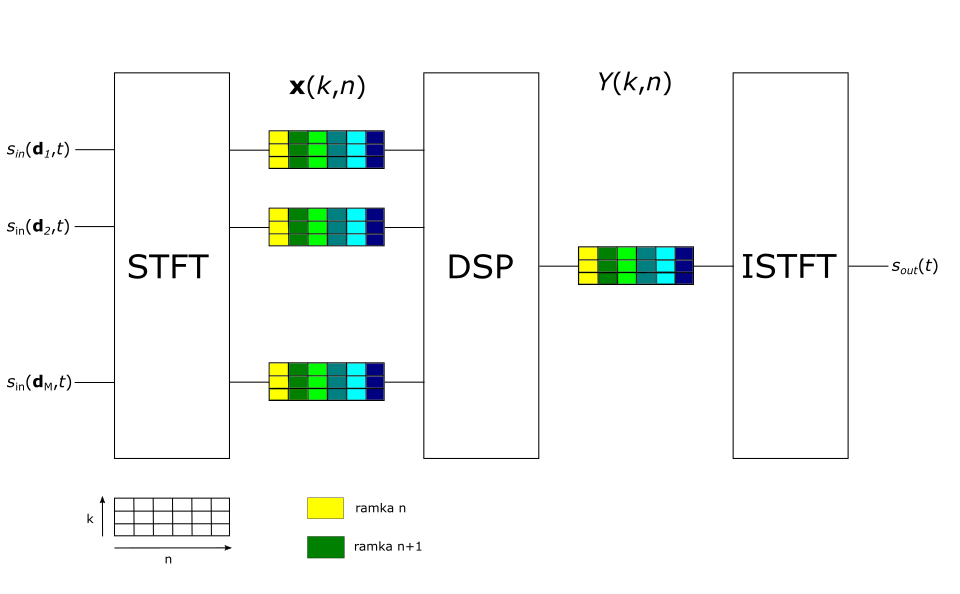
\includegraphics[width=\textwidth]{Images/processing.png}
    \caption{Schemat przetwarzania}
    \label{fig:processing}
\end{figure}

\noindent Na rysunku \ref{fig:processing} blok oznaczony jako automatyczna kontrola głośności zawiera w sobie operacje obliczenia PSD, estymacji DOA, wyznaczania współczynników i filtracji przy użyciu LCMV. Jest więc równoznaczny z diagramem \ref{fig:block_diagram}.



\chapter{Testy}
\label{chapter-5}
\section{Konfiguracja}
Dla celów testów przyjęto pewne sztywne założenia. Jako prędkość dzwięku przyjmuje się $343 \dfrac{m}{s}$ Wszystkie testy są przeprowadzane na sygnałach mowy próbkowanych na częstotliwości 4kHz. STFT i ISTFT jest obliczane przy pomocy okna hanninga \cite{hann} ze współczynnikiem nachodzenia okien(ang. overlap) 50$\%$. Jako okno przestrzenne wspomniane w \ref{alg:gprim} także przyjęto okno hanninga o szerokości $20^{\circ}$. Liczba ramek $N$, z których wyliczana jest macierz PSD jest równa 100.Aktualizacja DOA odbywa się co 10 próbek. Współczynniki $\alpha_{\mathrm{LT}}$ i $\alpha_{G}$ mają wartości 0.9. Jako macierz mikrofonową przyjęto kwadratową strukturę o liczbie mikrofonów $M=16$ o równomiernej odegłości między mikrofonami równej $\delta d = 1cm$. Na potrzeby niektórych eksperymentów odległość między mikrofonami była zwiększana.

W eksperymentach, w których włączony jest pogłos symulowany jest pokój o wymiarach 7m x 5m x 3m. Macierz umieszczona jest w punkcie $[2,2,1.6]$ a mówcy znajdują się w odległości 1.5m od niej. Ilustracja znajduje się na rysunku \ref{fig:room}.

\begin{figure}[h!]
    \centering
    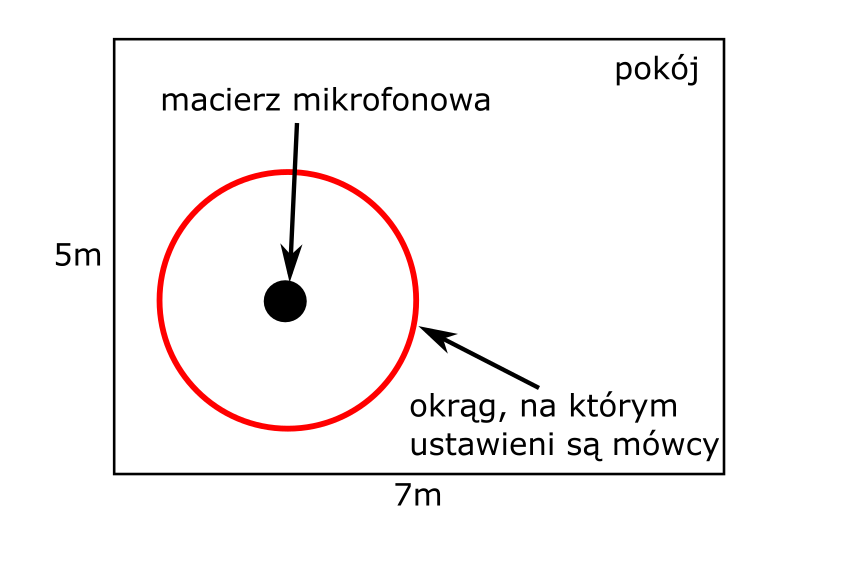
\includegraphics[width=0.4\textwidth]{Images/room.png}
    \caption{Symulowany Pokój}
    \label{fig:room}
\end{figure}

\begin{figure}[h!]
    \centering
    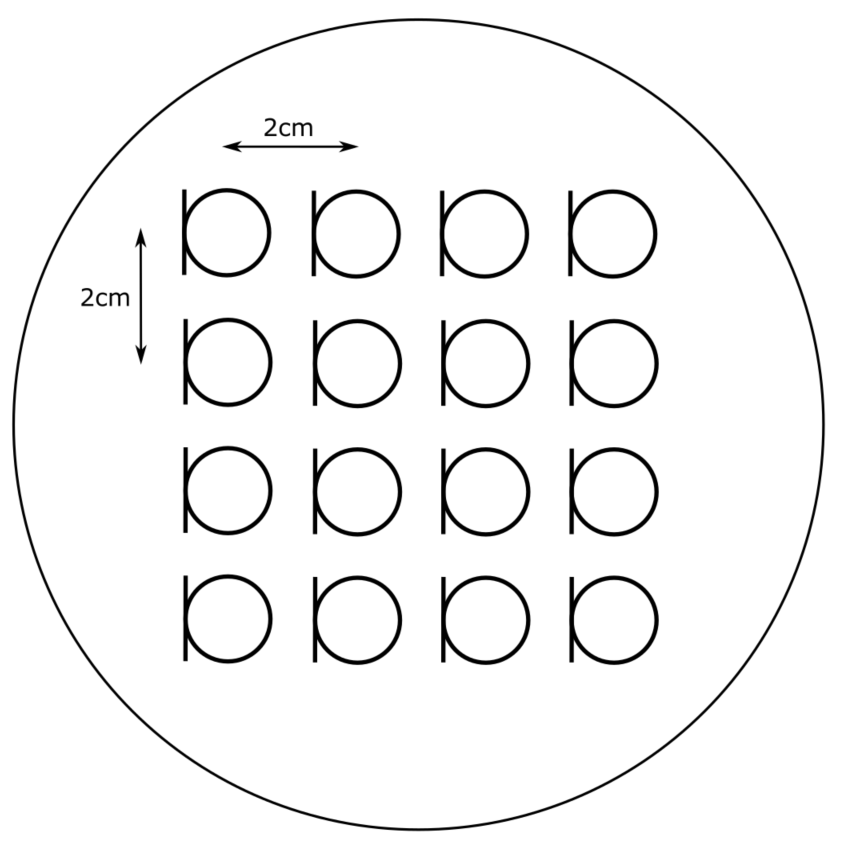
\includegraphics[width=0.4\textwidth]{Images/microphone.png}
    \caption{Macierz Mikrofonowa}
    \label{fig:microphone}
\end{figure}

Jako zakłócenie do usunięcia wybrano biały szum. Jego macierz PSD może być zapisana jako:

W sekcjach poniżej kolejno opisywane są wykonywane testy i doświadczenia.

\section{Charakterystyka kierunkowa filtra LCMV}

Poniżej przedstawiono wykresy charakterystyki kierunkowej dla filtra LCMV o następujących parametrach:

\begin{itemize}
    \item $\theta_{0}=30^{\circ}, \,
    \theta_{1}=120^{\circ}, \,
    \theta_{2}=300^{\circ}$
    \item $G(\theta_{0})=4, \,
    G(\theta_{1})=2, \,
    G(\theta_{2})=1$
\end{itemize}
\noindent dla częstotliwości 100Hz, 500Hz i 2kHz.

\begin{figure}[h!]
    \centering
    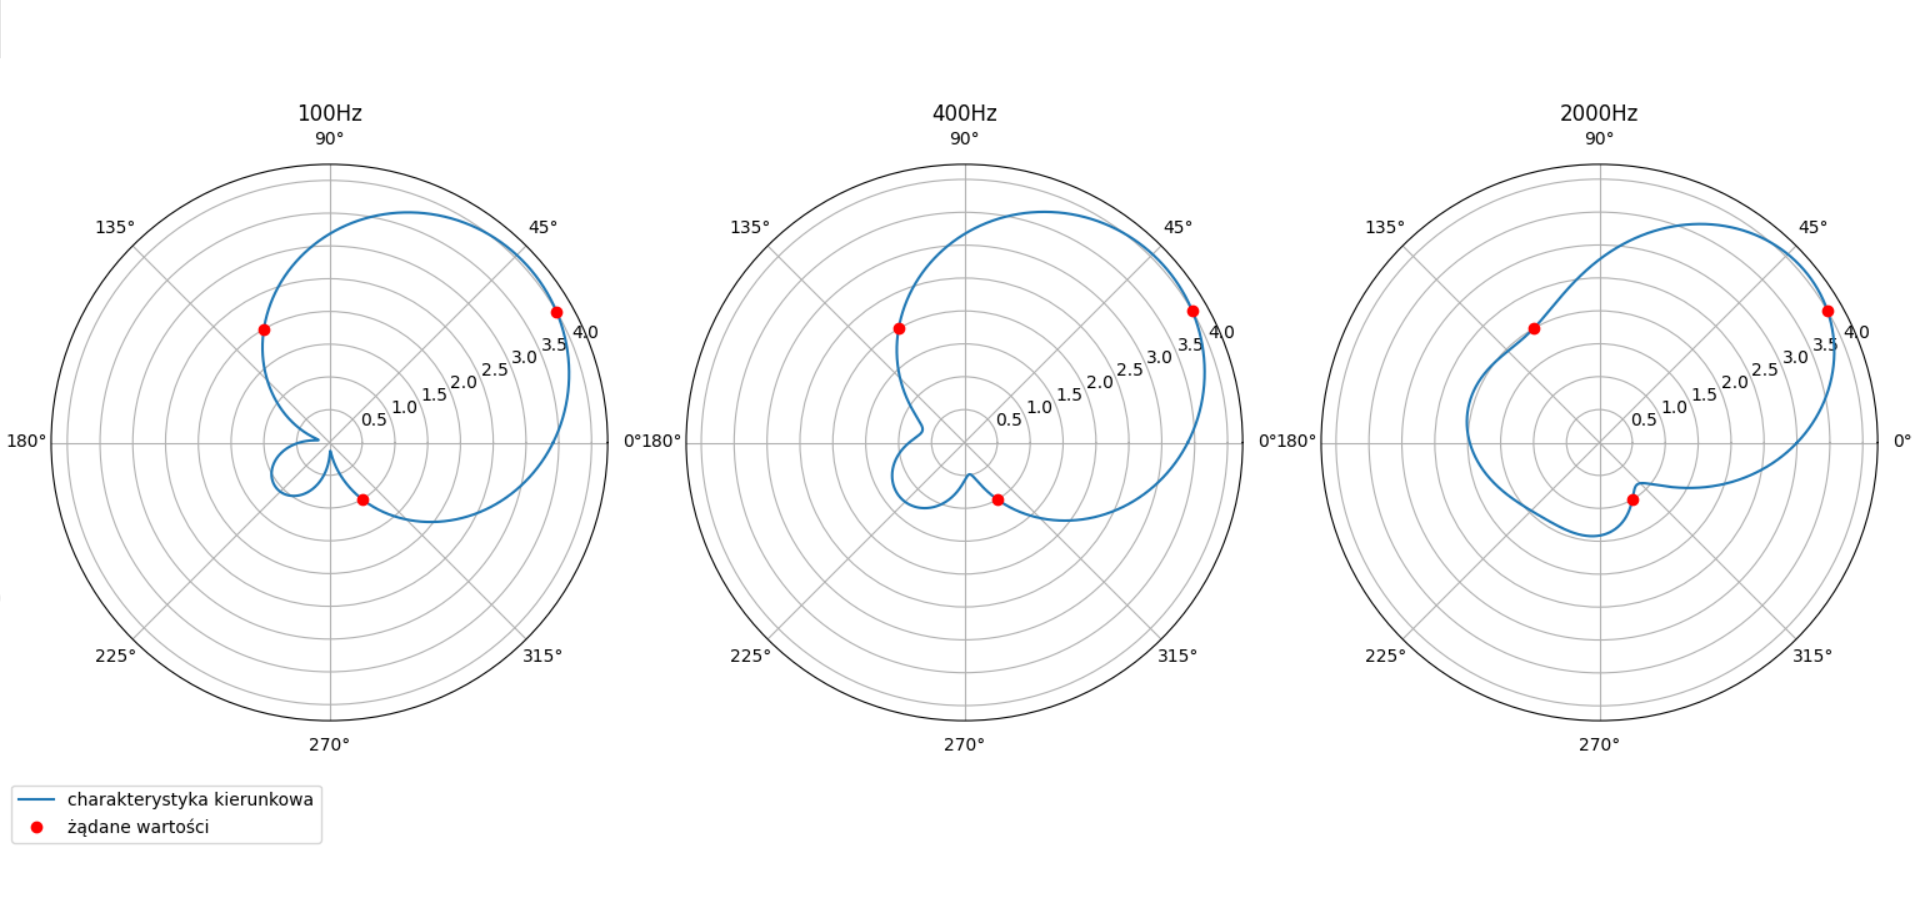
\includegraphics[width=\textwidth]{Images/directivity0.02m.png}
    \caption{Charakterystyka kierunkowa dla $\Delta d = 2cm$}
    \label{fig:directivity0.02}
\end{figure}

\noindent Załączony obrazek \ref{fig:directivity0.02} pokazuje, że filtr prawidłowo generuje wymuszenia w określonych kierunkach. Właściwości usuwania tła akustycznego zostaną sprawdzone w kolejnych sekcjach.

\noindent Zgodnie z teorią przedstawioną w \cite{mccowan2001} wraz ze wzrostem stosunku $\dfrac{\Delta d}{\lambda}$, gdzie $\lambda$ to długość fali, rośnie kierunkowość filtru. Prowadzi to do sytuacji, w której maksima są bardzo wąskie i wartość charakterystyki kierunkowej silnie fluktuuje w dziedzinie kątów. Nieznaczny błąd estymacji kierunku nadchodzenia fali może więc prowadzić do fatalnych skutków. Zjawisko pojawiania się dużej liczby minimów i maksimów nazywane jest aliasingiem przestrzennym. Zachodzi dla $\Delta d > \dfrac{\lambda}{2}$. Przy założonej prędkości dzwięku dla częstotliwości $f = 4kHz$ granica aliasingu przestrzennego wystąpi dla $\Delta d \approx 4cm $.Dlatego właśnie zdecydowano się wybrać bezpieczną odległość między mikrofonami $\Delta d = 2cm$.

\noindent Warte pokazania są wykresy takich samych filtrów jeśli mikrofony byłyby oddalone od siebie odpowiednio o $\Delta d = 20cm$ i $\Delta d = 2m$:

\begin{figure}[h!]
    \centering
    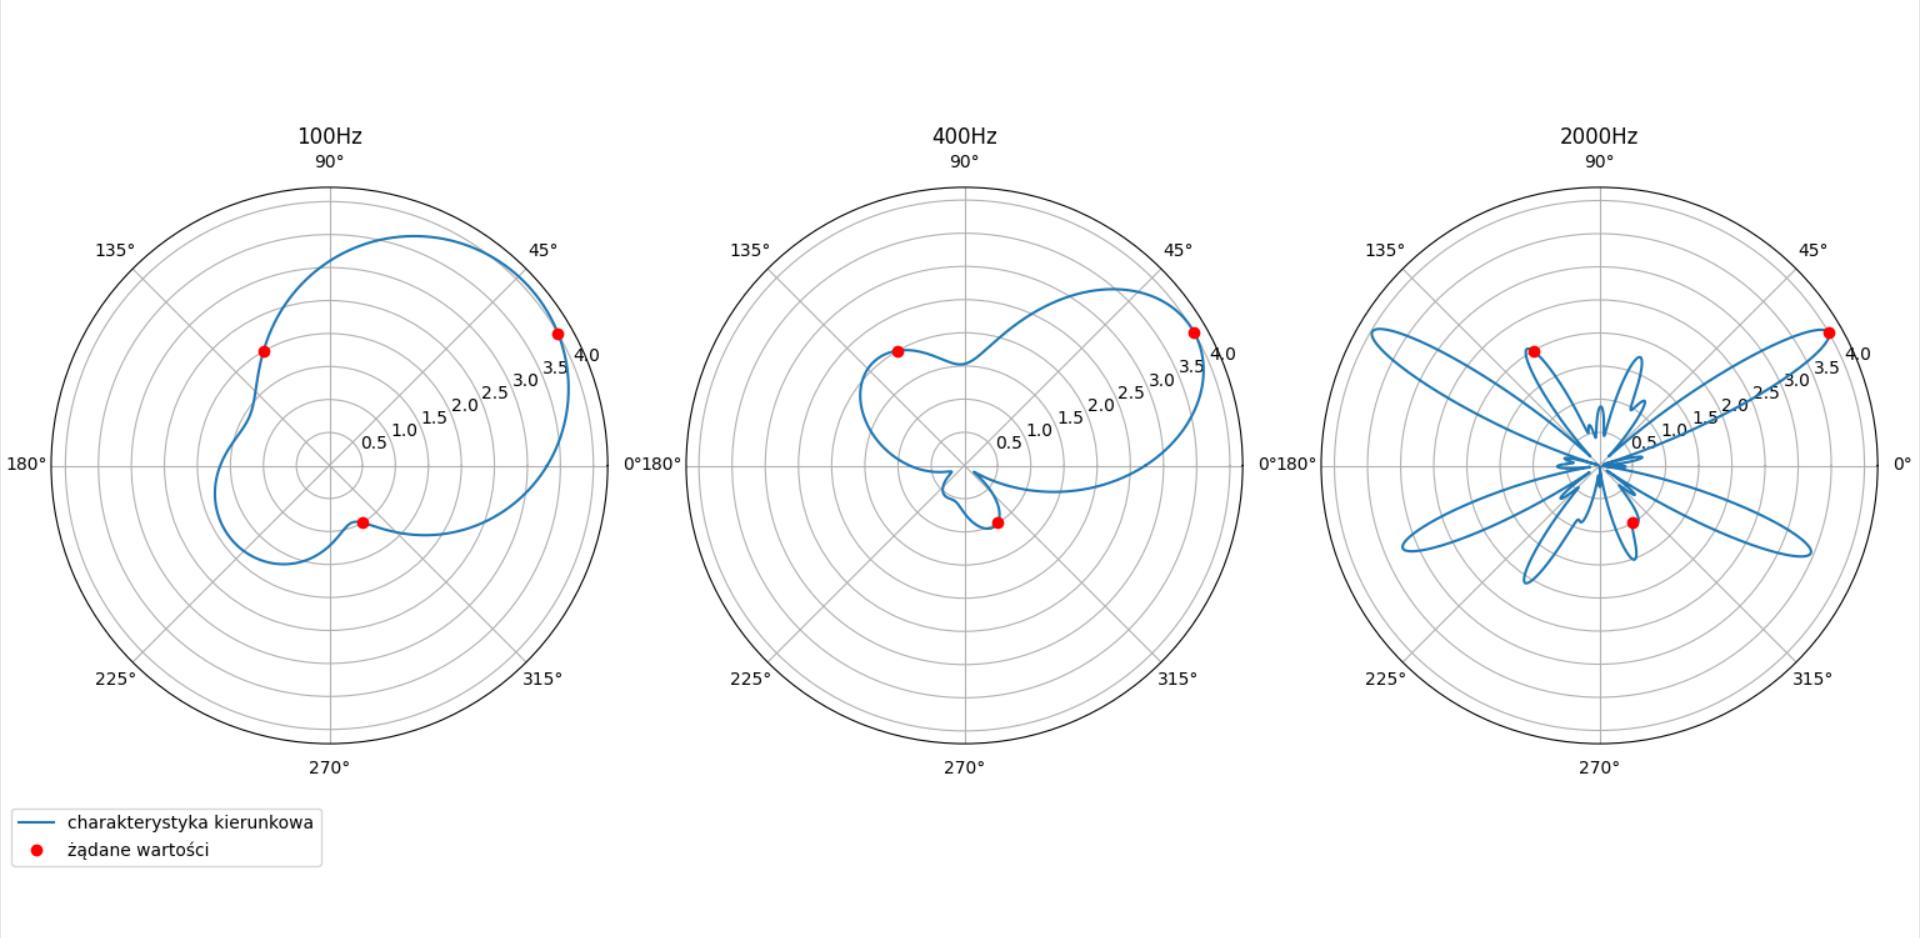
\includegraphics[width=\textwidth]{Images/directivity0.2m.png}
    \caption{Charakterystyka kierunkowa dla $\Delta d = 20cm$}
    \label{fig:directivity0.2}
\end{figure}

\begin{figure}[h!]
    \centering
    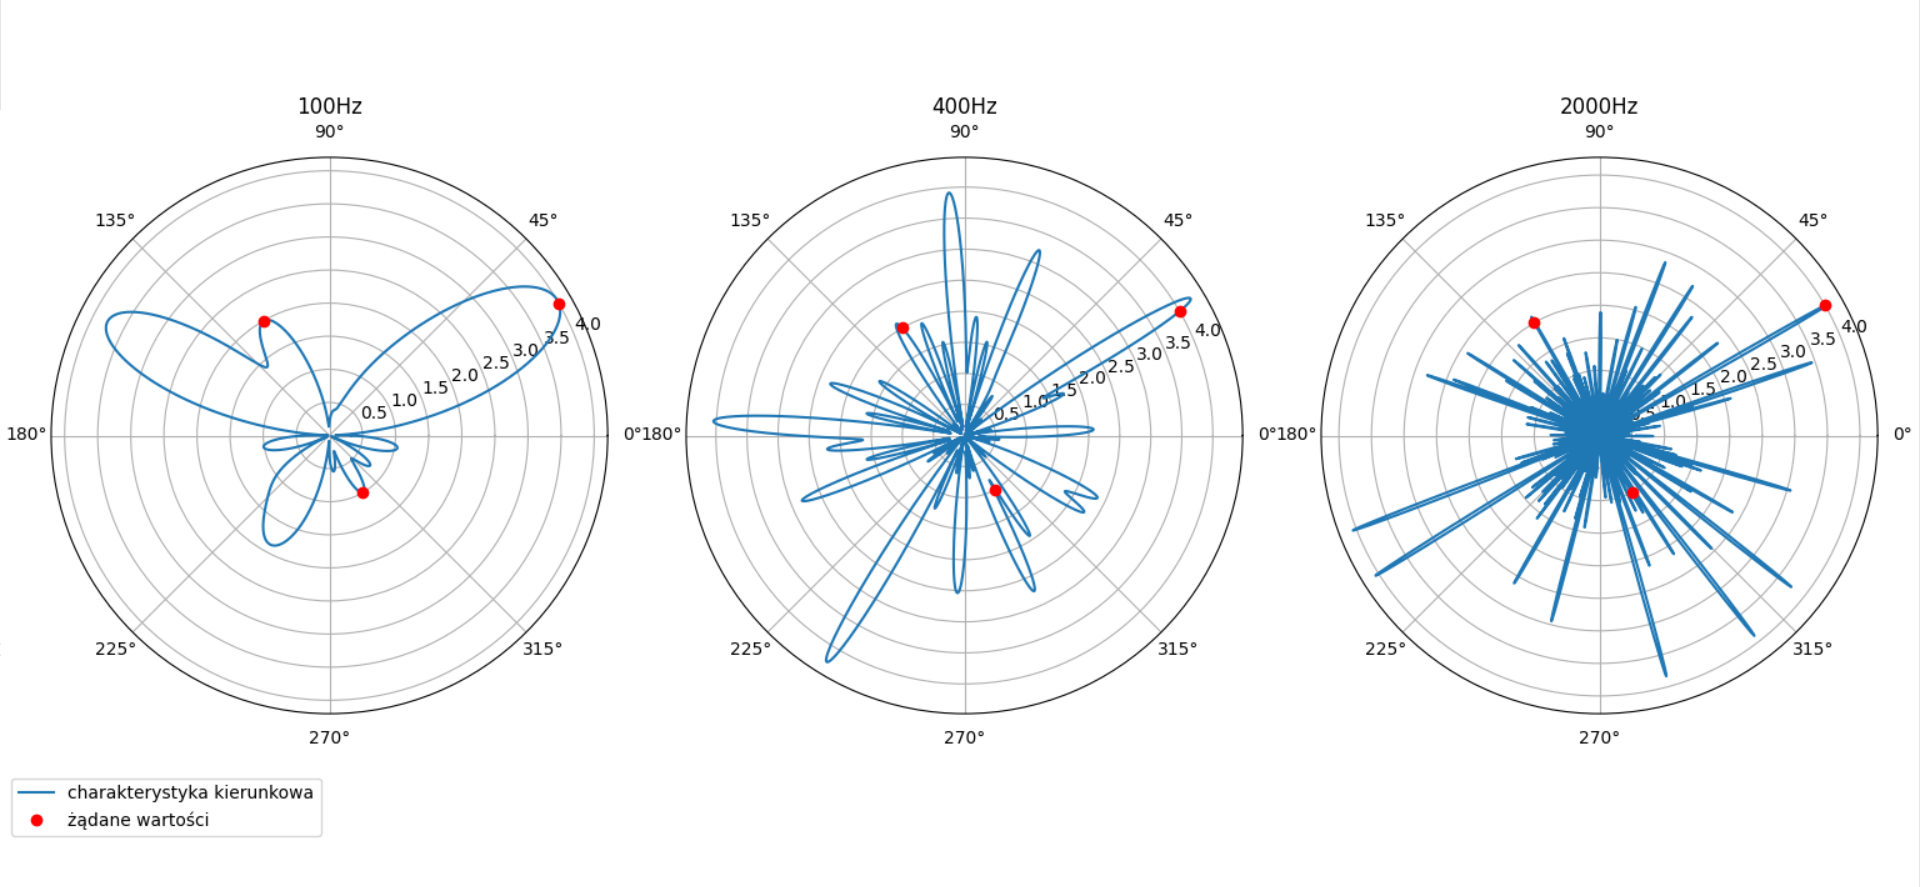
\includegraphics[width=\textwidth]{Images/directivity2m.png}
    \caption{Charakterystyka kierunkowa dla $\Delta d = 2m$}
    \label{fig:directivity2}
\end{figure}

\newpage

\section{Ewaluacja algorytmu MUSIC}

\noindent W celu sprawdzenia działania zaproponowanego algorytmu MUSIC sprawdzone są różne warianty rozłożenia mówców:

\begin{itemize}
    \item Jeden mówca usytuowany na kącie $\theta_{0} = 78^{\circ}$

    \item Trzech mówców usytuowanych na kątach $\theta_{0} = 78^{\circ}, \, \theta_{1} = 192^{\circ}, \, \theta_{2} = 301^{\circ}$
    
\end{itemize}

\noindent Wszystkie powyższe scenariusze będą powtórzone dla następjących konfiguracji odległości między mikrofonami, wartości stosunku sygnału do szumu i obecności pogłosu:

\begin{itemize}
    \item $\mathrm{SNR}=10\mathrm{dB}$ 
    \item $\mathrm{SNR}=-10\mathrm{dB}$
    \item $\mathrm{SNR}=10\mathrm{dB}, \, $ z pogłosem
\end{itemize}

\noindent Te wartości zostały sprawdzone dla $\Delta d = 2cm$ i $\Delta d = 20cm$ dla porównania. Wygenerowane wykresy przedstawiające znalezione DOA mogą być znalezione w tekście jako załączniki \ref{fig:music_10db_2cm}-\ref{fig:music_10db_20cm_reverb}. Na przedstawionych wykresach po lewej stronie znajduje się efekt działania dla jednego źródła a po prawej dla trzech źródeł.

\begin{figure}[H]
    \centering
    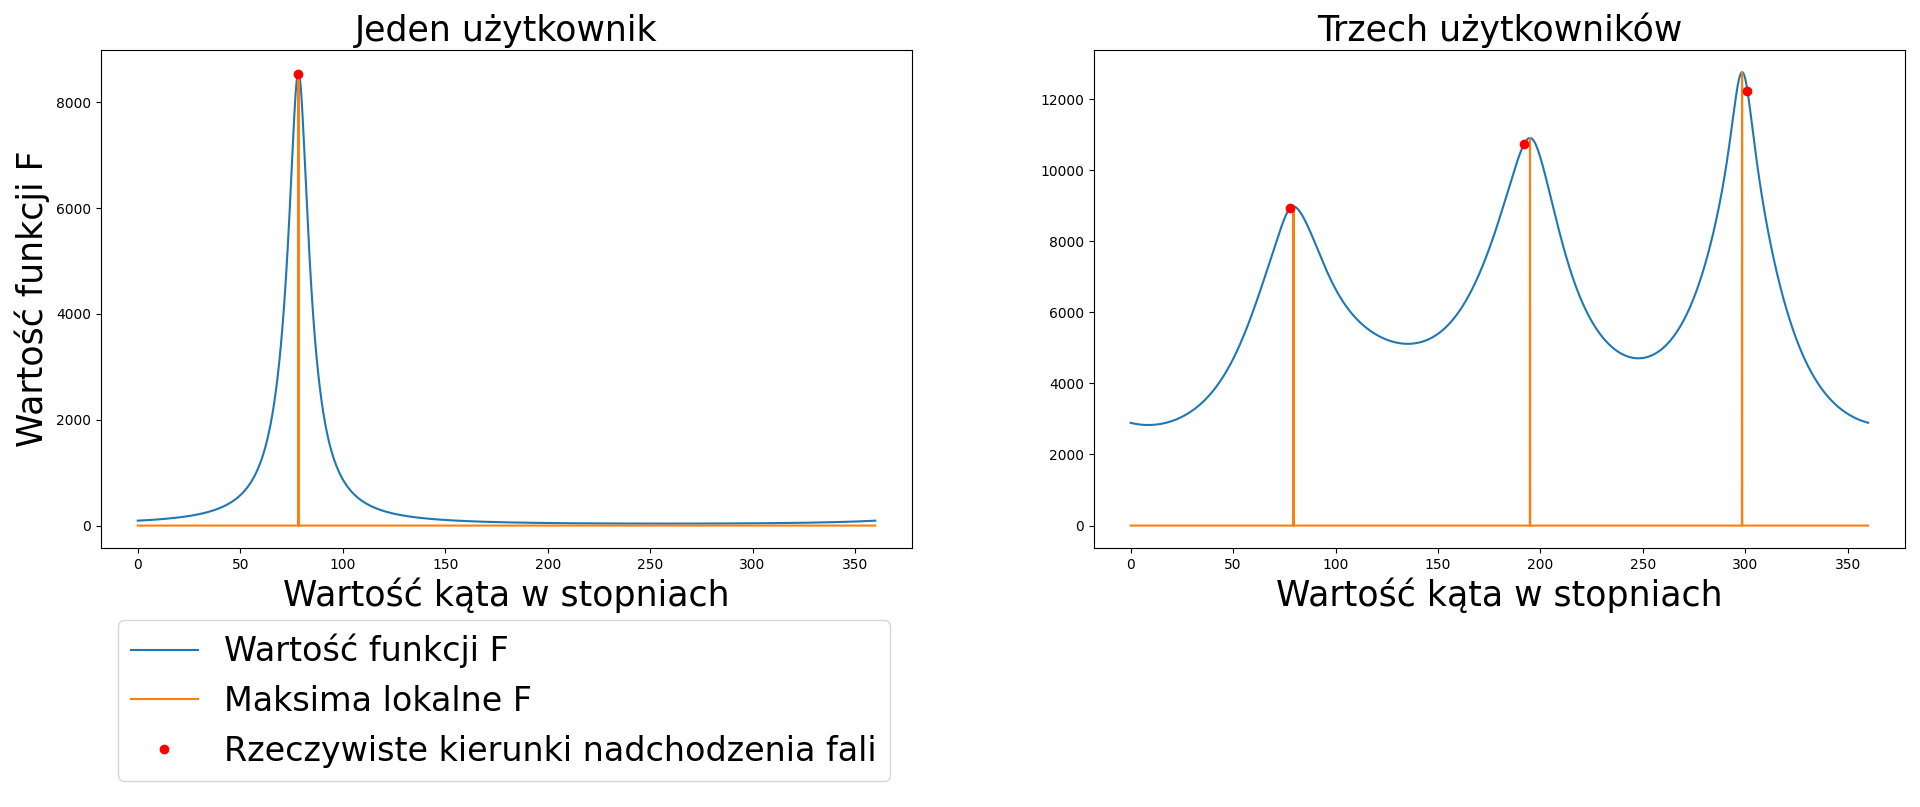
\includegraphics[width=0.85\textwidth]{Images/music_10db.png}
    \caption{$\mathrm{SNR}=10\mathrm{dB}, \, \Delta d = 2cm$}
    \label{fig:music_10db_2cm}
\end{figure}

\begin{figure}[H]
    \centering
    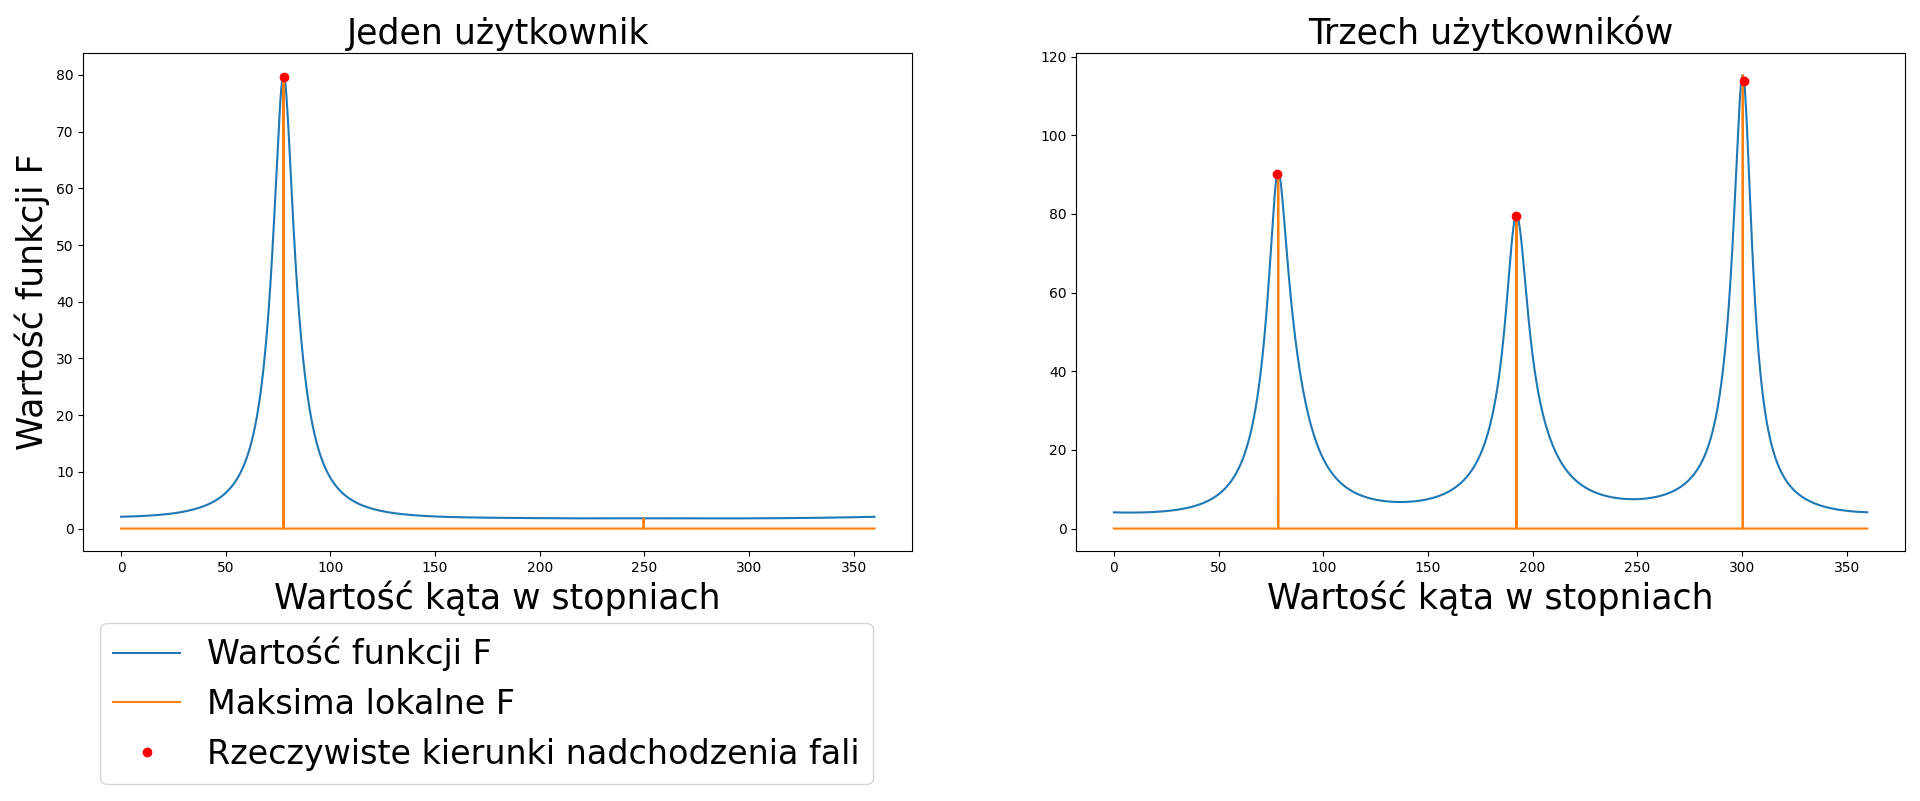
\includegraphics[width=0.85\textwidth]{Images/music_-10db.png}
    \caption{$\mathrm{SNR}=-10\mathrm{dB}, \, \Delta d = 2cm$}
    \label{fig:music_-10db_2cm}
\end{figure}

\begin{figure}[H]
    \centering
    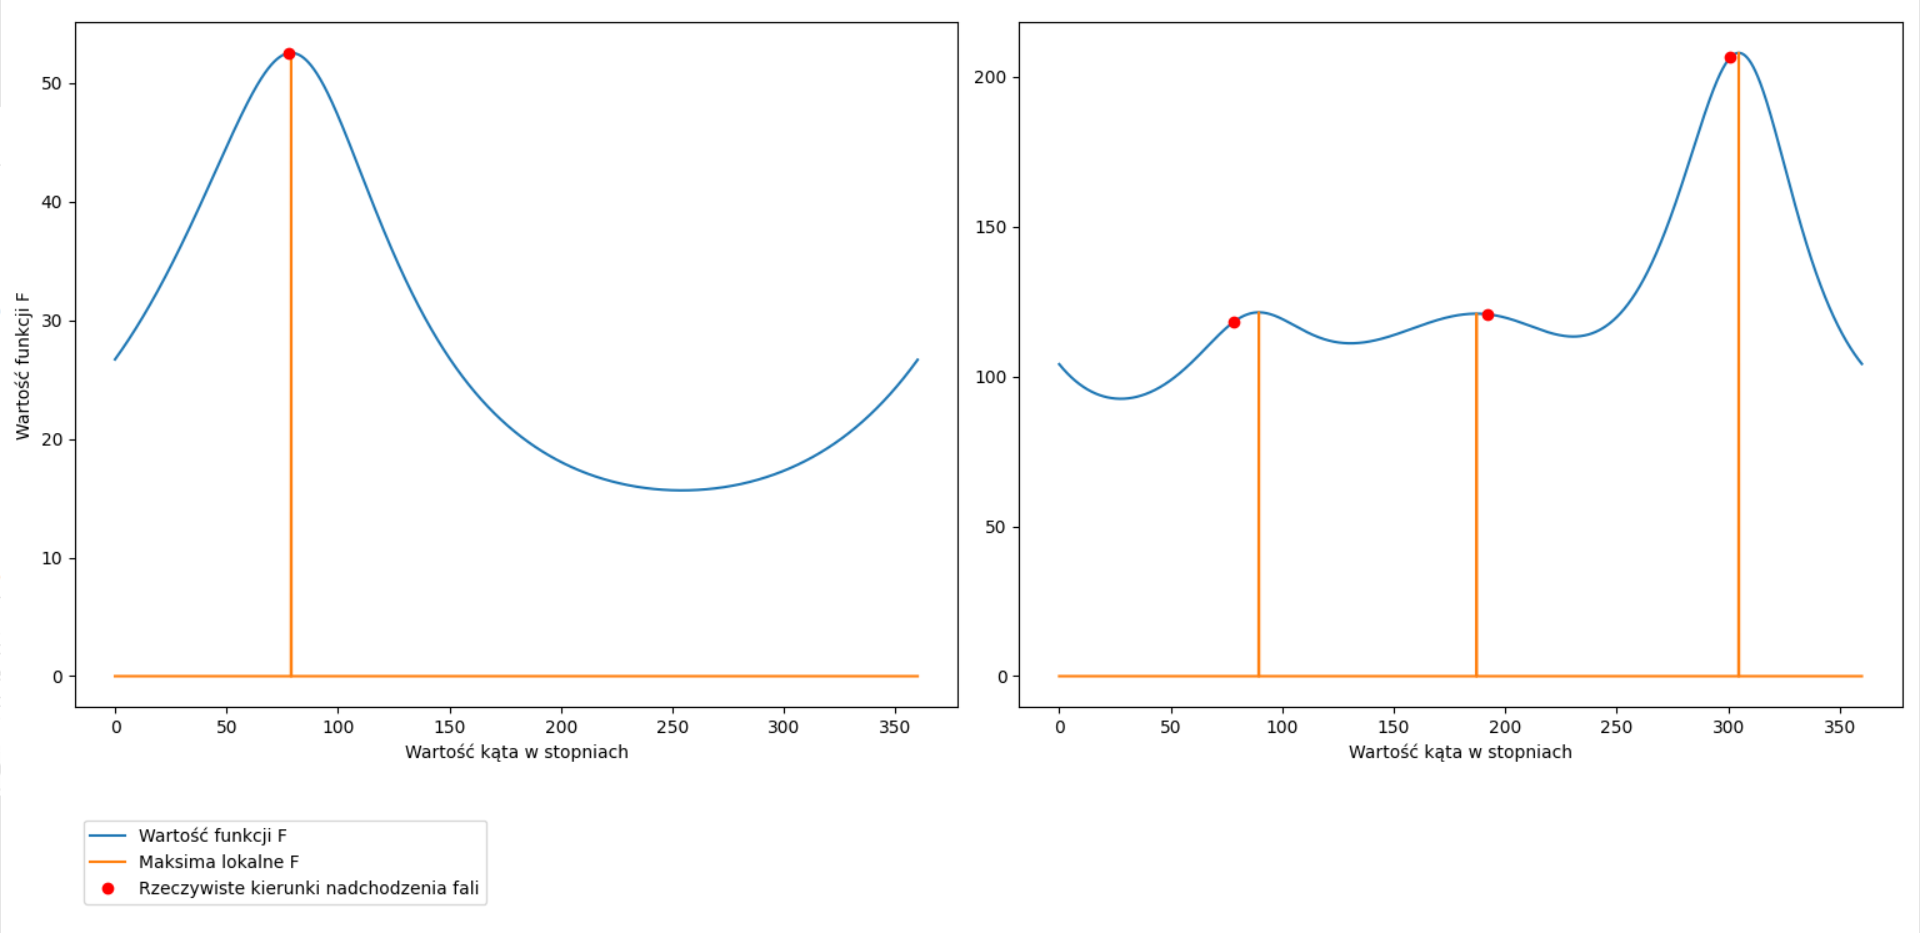
\includegraphics[width=0.85\textwidth]{Images/music_10db_reverb.png}
    \caption{$\mathrm{SNR}=10\mathrm{dB}, \, \Delta d = 2cm$ z pogłosem}
    \label{fig:music_10db_2cm_reverb}
\end{figure}

\begin{figure}[H]
    \centering
    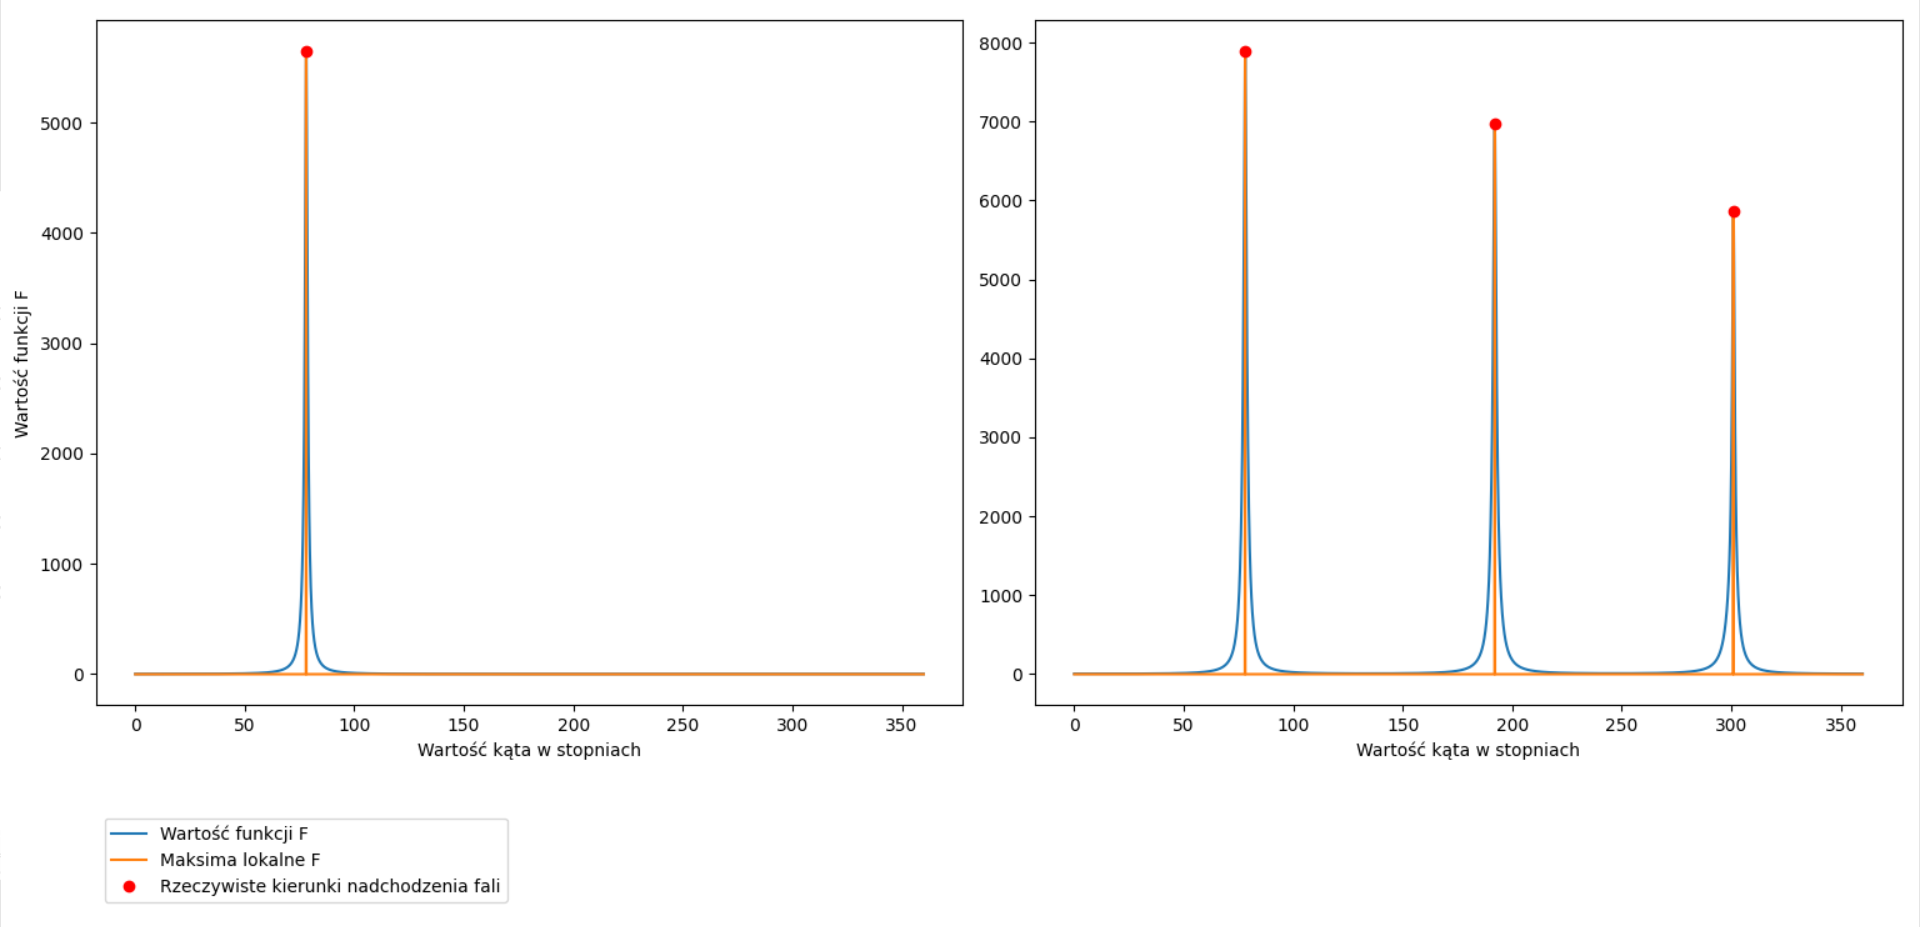
\includegraphics[width=0.85\textwidth]{Images/music_10db_0.2m.png}
    \caption{$\mathrm{SNR}=10\mathrm{dB}, \, \Delta d = 20cm$}
    \label{fig:music_10db_20cm}
\end{figure}

\begin{figure}[H]
    \centering
    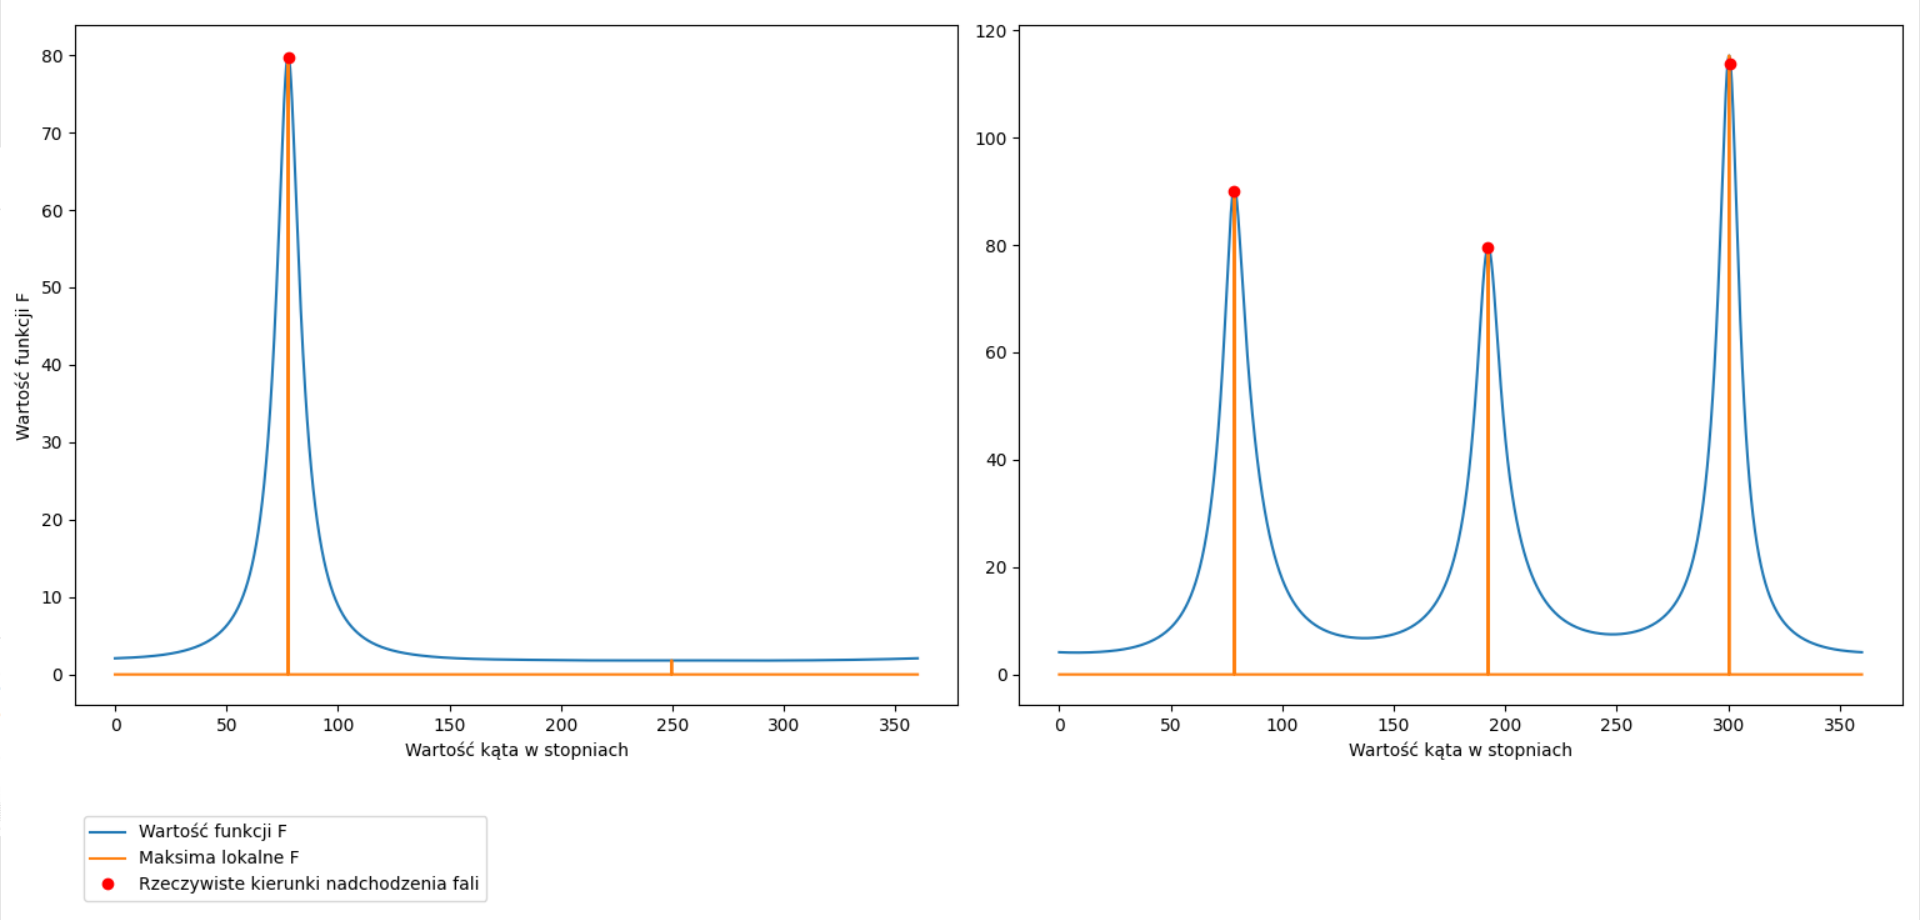
\includegraphics[width=0.85\textwidth]{Images/music_-10db_0.2m.png}
    \caption{$\mathrm{SNR}=-10\mathrm{dB}, \, \Delta d = 20cm$}
    \label{fig:music_-10db_20cm}
\end{figure}

\begin{figure}[H]
    \centering
    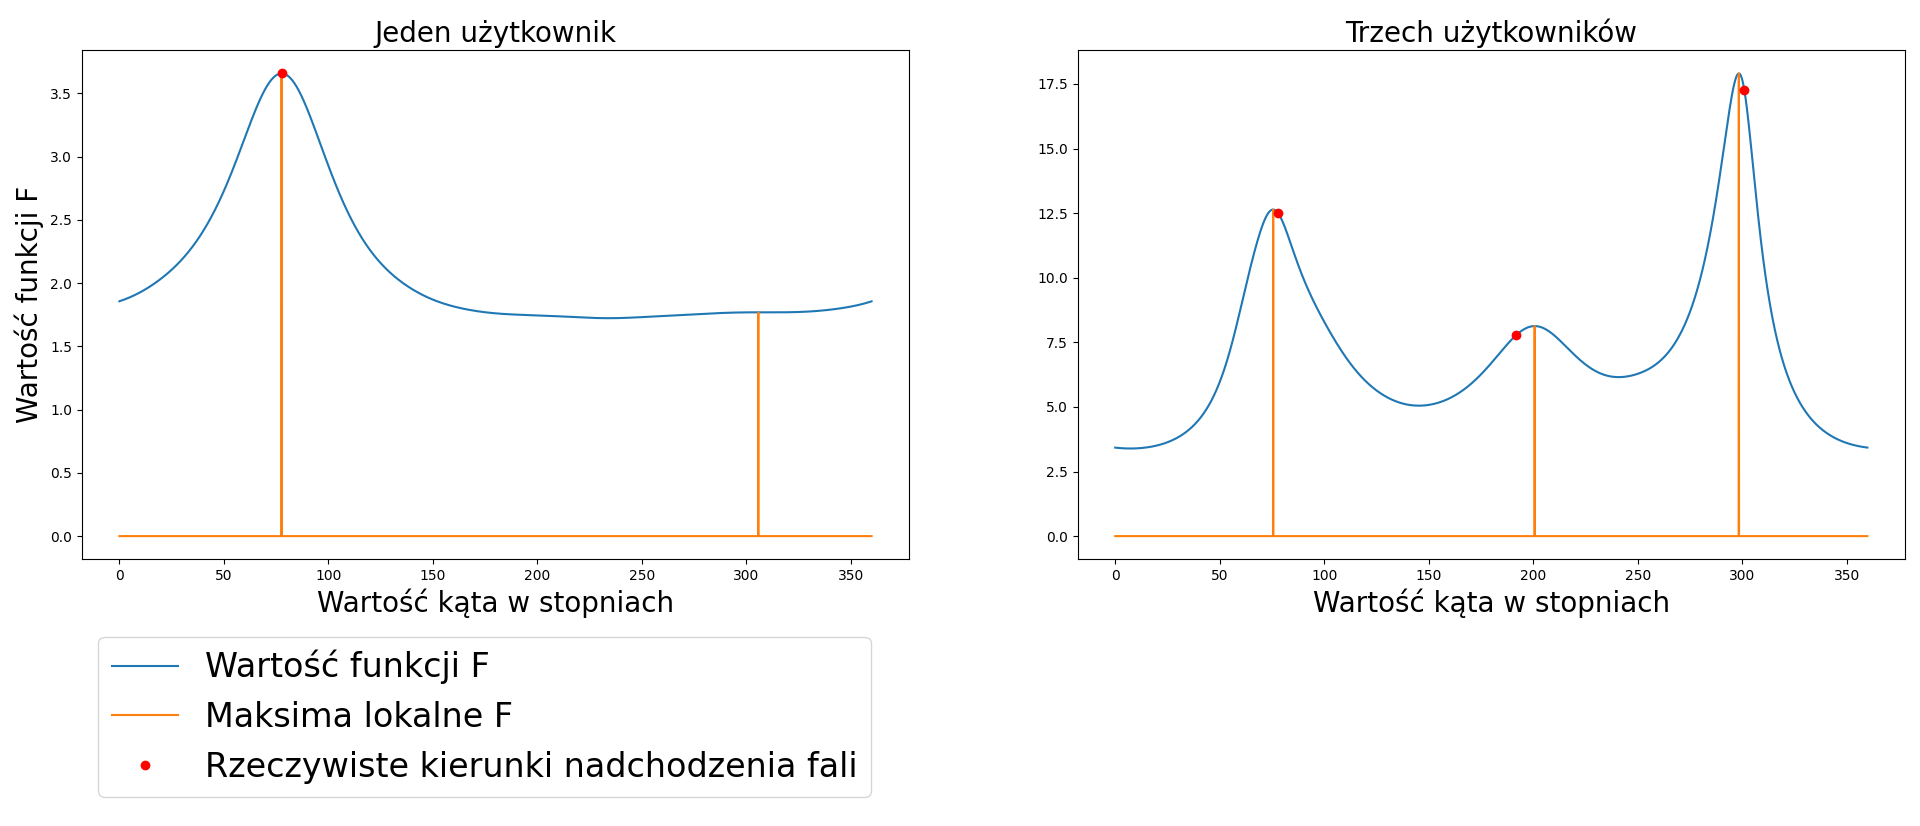
\includegraphics[width=0.85\textwidth]{Images/music_10db_reverb_0.2m.png}
    \caption{$\mathrm{SNR}=10\mathrm{dB}, \, \Delta d = 20cm$ z pogłosem}
    \label{fig:music_10db_20cm_reverb}
\end{figure}

Wyniki dotyczące wpływu szumu nie zaskakują- algorytm działa mniej dokładnie dla niskiego SNR. To samo dotyczy pogłosu, użyty algorytm nie jest odporny na tego typu zakłócenia. Pojawiające się odbite fale wewnątrzpokoju czynią maksima mniej wybitnymi. Najbardziej interesująca obserwacja zdaniem autora pracy to wpływ odległości między mikrofonami. Większa odległość powoduje większą kierunkowość co przekłada się na dokładniejszą estymację. Dla rozłożenia $\Delta \d = 20cm$ i szumie $\mathrm{SNR}=-10\mathrm{dB}$ udaje się dokładnie wyestomować wszystkie trzy kierunki. Dla tego samego stosunku sygnału do szumu i $\Delta d = 2cm$ algorytm estymuje tylko dwa kierunki i to bardzo niedokładnie. Do dalszych testów wybrano jednak system ze stosunkiem sygnału do szumu na poziomie 10dB a mówcy są dość daleko od siebie.Zbytnia kierunkowość powoduje duże problemy z zastosowaniem filtra LCMV i nawet bardzo dokładna estymacja nie rekompensuje tych strat. .Doświadczenia empiryczne pokazały, że cały system działa lepiej dla $\Delta d = 2cm$.

\newpage

\section{Wizualizacja Działania AGC}

W celu oceny działania kontroli głośności i zrozumienia połączeń pomiędzy funkcjami $\Psi$, $\Psi_{\mathrm(LT)}$, $G'$, $\widehat(G)$. 

\section{Testy całego systemy}

Testy całego systemu sprawdzają kilka różnych aspektów projektu inżynierskiego. Są to:

\begin{itemize}
    \item Stosunek sygnału do szumu(SNR)
    \item Ocena działania systemu dla jednego użytkownika
    \item Ocena działania systemu dla wielu użytkowników
    \item Ewaluacja wpływu poruszania się źródła na działanie algorytmu
    \item Sprawdzenie wpływu pogłosu na jakość przetwarzania
    
\end{itemize}
\subsection{SNR}

Obliczenie SNR dla systemu jest obliczane zarówno dla systemu z pojedynczym użytkownikiem jak i z trzema użytkownikami. Aby obliczyć SNR zakłada się, że $\bm{\mathrm}g = \{1,..,1\}$ dla każdego indeksu czasowego. Oznacza to wyłączenie AGC. Z włączonym AGC następowałyby zmiany lokalnej amplitudy sygnału uniemożliwiając sensowny pomiar SNR. Wszystkie pomiary SNR podaje się w skali logarytmicznej.

\noindent Zastosowano następującą normę pomiaru poprawy SNR:
\begin{equation}
    \label{delta_SNR}
    \Delta \mathrm{SNR} = \mathrm{SNR}_{\mathrm{output}} - \mathrm{SNR}_{\mathrm{input}}
\end{equation}

\noindent Gdzie SNR na wejściu $\mathrm{SNR}_{\mathrm{input}}$ jest znane a mając do dyspozycji niezaszumiony sygnał referencyjny $s_{\mathrm{ref}}(n)$ i sygnał zaszumiony $s_{\mathrm{noisy}}(n)$ można także obliczyć stosunek sygnału do szumu dla $N$ próbek sygnału jako:

\begin{equation}
    \label{SNR}
    \mathrm{SNR} = 10 \log \sum_{n=1}^{N}\left(
    \dfrac
    {s_{\mathrm{ref}}(n)}
    {s_{\mathrm{ref}}(n)-s_{\mathrm{noisy}}(n)} \right)^{2}
\end{equation}
\noindent Taki pomysł obliczania SNR zaczerpnięto luźno z \cite{Virtanen2006}.

\noindent Uzyskano następujące wyniki:
\begin{itemize}
    \item Pojedynczy użytkownik: $\mathrm{SNR} \approx 12dB$ 
    \item Trzech użytkowników: $\mathrm{SNR} \approx 6dB$
\end{itemize}

\noindent Wykresy przedstawiające sygnały przed i po odszumaniu przedstawiono na \ref{fig:snr_boost}

\begin{figure}[h!]
    \centering
    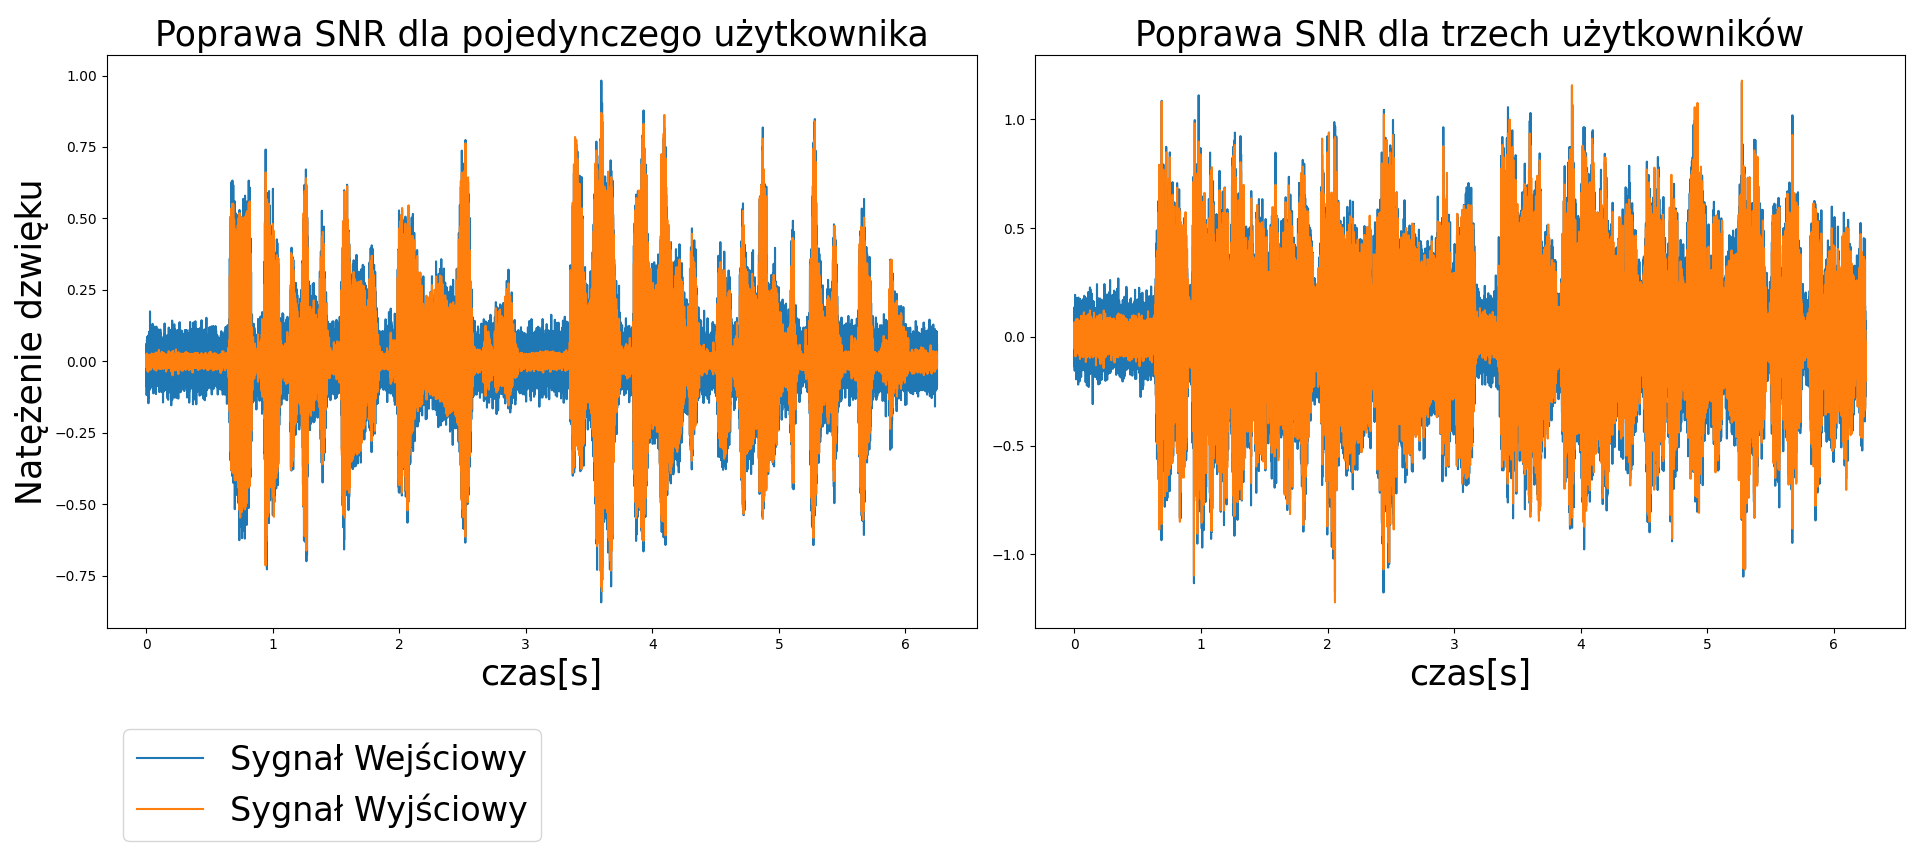
\includegraphics[width=\textwidth]{Images/snr_boost.png}
    \caption{Poprawa SNR}
    \label{fig:snr_boost}
\end{figure}

\subsection{Działanie algorytmu dla pojedynczego użytkownika}

Ocenę algorytmu dla pojedynczego użytkownika przeprowadzono w warunkach gdzie użytkownik jest ustawiony na $\theta_{0}=78^{\circ}$. Nagrany sygnał ma długość 50000 próbek co przekłada się na nieco ponad 6 sekund.
\noindent W celu oceny jakości działania sprawdza się dwa warianty zmian sygnału w czasie:
\begin{itemize}
    \item Dziesięciokrotny wykładniczy wzrost amplitudy w czasie trwania sygnału
    \item Dziesięciokrotny wykładniczy spadek amplitudy w czasie trwania sygnału
\end{itemize}

\noindent W obu przypadkach początkowy SNR wynosi 10dB. Wyniki eksperymentu przedstawiono na wykresach \ref{fig:single_user_increasing} i \ref{fig:single_user_decreasing}

\begin{figure}[h]
    \centering
    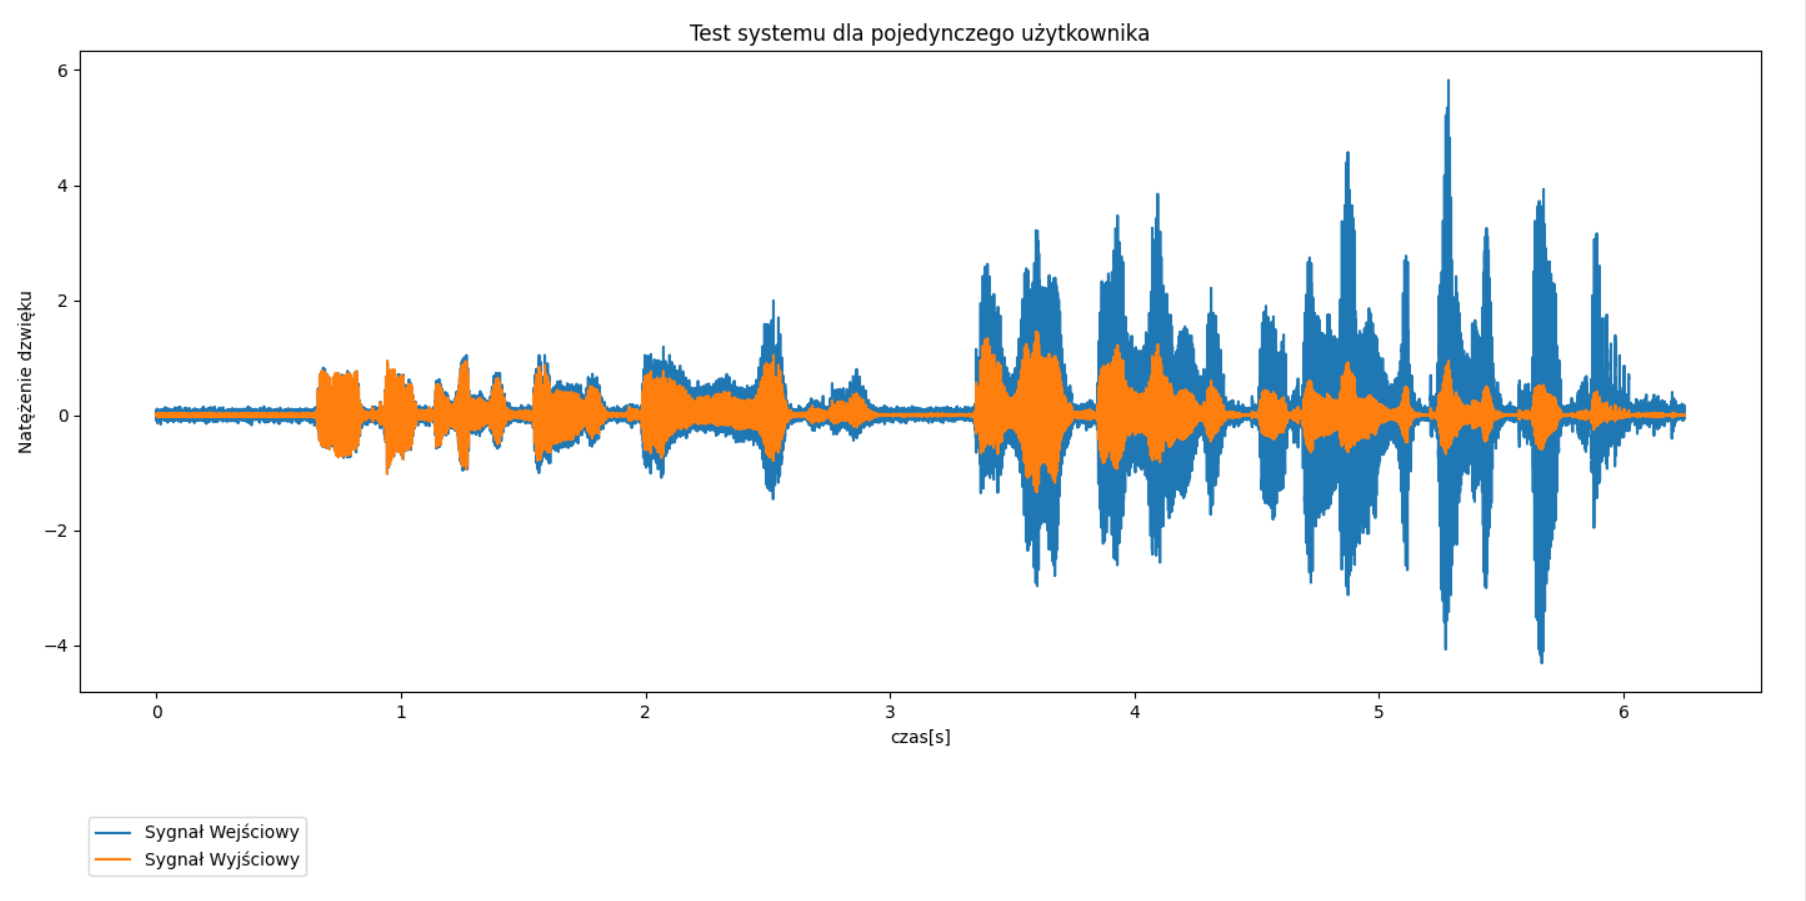
\includegraphics[width=\textwidth]{Images/single_user_increasing.png}
    \caption{Wzrost amplitudy sygnału dla pojedynczego użytkownika}
    \label{fig:single_user_increasing}
\end{figure}

\begin{figure}
    \centering
    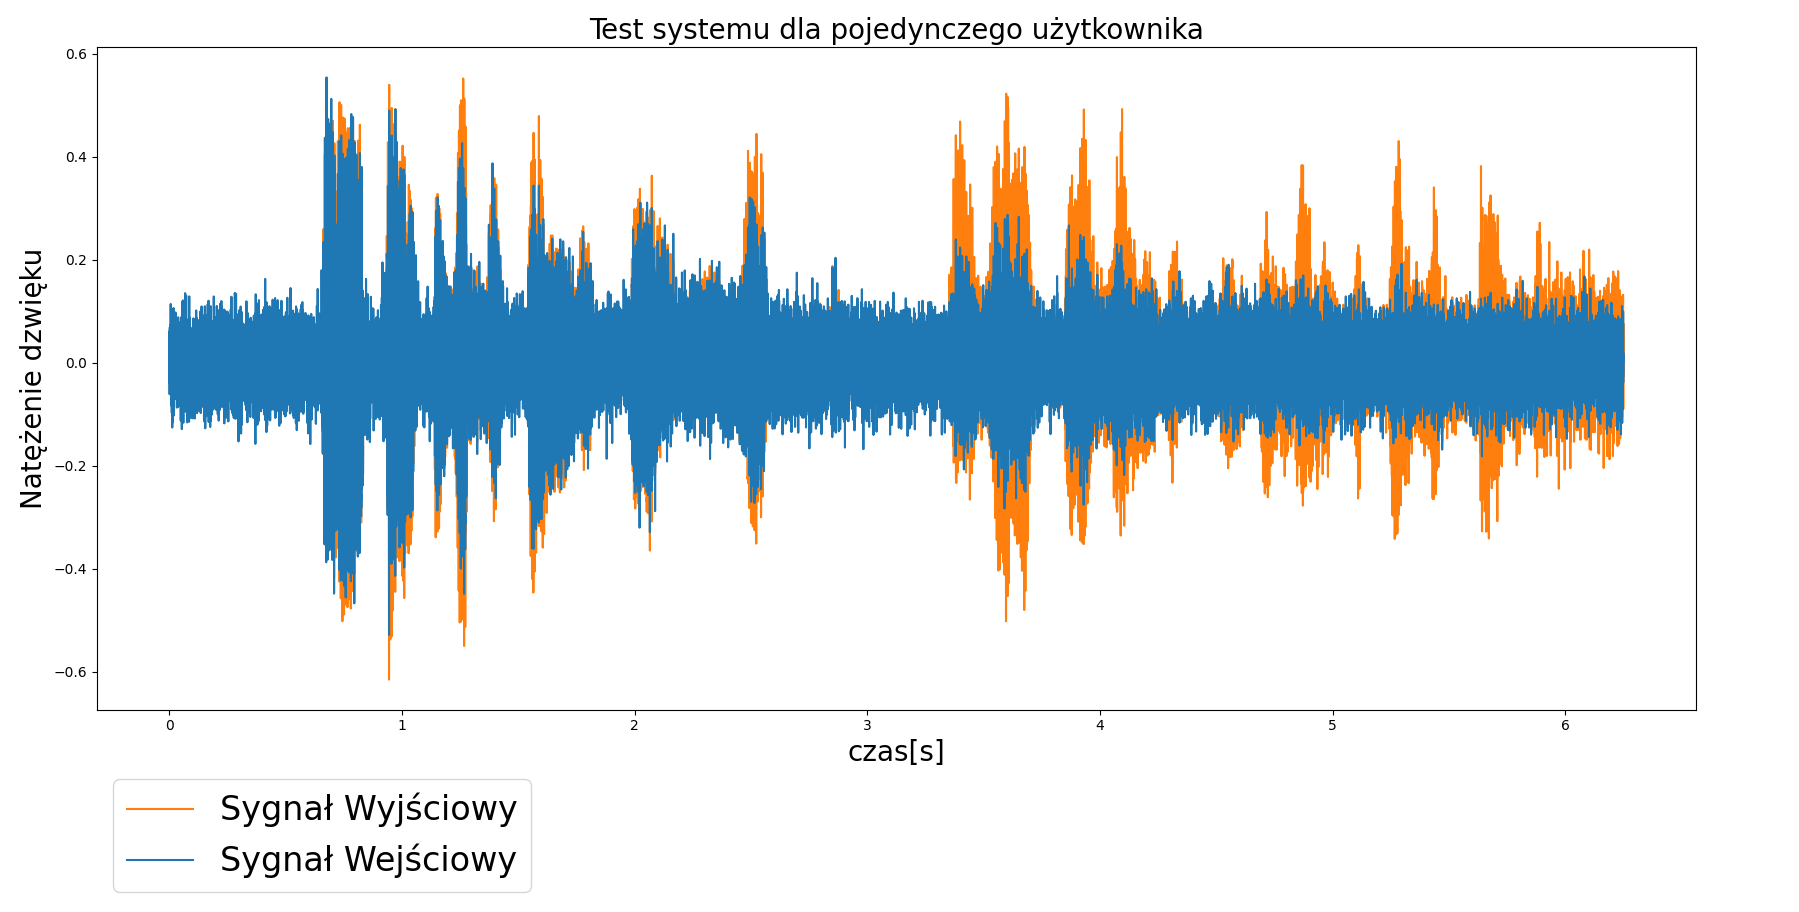
\includegraphics[width=\textwidth]{Images/single_user_decreasing.png}
    \caption{Spadek amplitudy sygnału dla pojedynczego użytkownika}
    \label{fig:single_user_decreasing}
\end{figure}

\noindent Wyniki wymagają krótkiego komentarza. Widoczne jest, że w obu przypadkach mimo, że amplituda sygnału wejściowego silnie zmienia się w czasie, sygnał wyjściowy utrzymuje względnie stały poziom obwiedni. Szczególnie interesujący jest fakt, że w przypadku słabnącego sygnały wejściowego wzmocnienie sygnału powoduje jego wyjście ponad poziom szumu.

\subsection{Działanie algorytmu dla wielu użytkowników}

W przypadku wielu użytkowników nie jest tak łatwo zaprezentować działanie algorytmu za pomocą wykresu wyjściowego. W celu oceny działania algorytmu konieczne będzie obejrzenie zależności wewnętrzych pomiędzy sygnałami $\Phi$, $\Phi_{\mathrm(LT_SLD)}$, $G'$, $\widehat{G}$. Co więcej zachęca się czytelnika pracy do zapoznania się z próbkami znajdującymi się na stronie...













\chapter{Podsumowanie}
\label{chapter-6}

Celem pracy inżynierskiej było napisanie algorytmu autmoatycznej kontroli głośności dla macierzy mikrofonowej z jednoczesnym tlumieniem tła akustycznego. Temat udało się zrealizować. Sposób działania algorytmu został zaczerpnięty z literatury, w dużej mierze z \cite{Braun2014}, \cite{Thiergart2013} i  \cite{Schmidt1986}. System napisano w języku python. Otrzymany algorytm przetwarza nagrania z macierzy mikrofonowej. Działanie algorytmu spełnia postawione założenia -steruje głośnością i tłumi zakłócenie jakim jest biały szum. Zdecydowano się zrealizować żądany system za pomocą filtru LCMV i algorytmu MUSIC.

Algorytm poddano licznym testom. Przetestowano wpływ czynników takich jak poziom szumu, ilość mówców, zmiennośc położenia mówców czy geometrię pokoju i mikrofonu na działanie zrealizowanego rozwiązania. Dokonano analizy otrzymanych wyników i wyciągnięto wnioski, które zostały opisane w rodziale \ref{chapter-5}. 

W planach autora pracy jest pogłębianie wiedzy na temat AGC i ulepszanie systemu. Plany te zakładają ulepszenie algorytmu estymacji DOA tak aby kierunki nadchodzenia fali były wykrywane dla sygnału składającego się ze źródeł położonych bliżej i dla mniejszej wartości stosunku sygnału do szumu. W planach jest także próba szybszej implementacji sprzętowej i uruchomienie algorytmu w czasie rzeczywistym.

%\bibliographystyle{}
%\bibliography{export}
\printbibliography

\appendix

%\chapter{Źródła pakietu Clicka FAMTAR}
\label{appendix-a}

\lstset{
language=C++,
basicstyle=\ttfamily\footnotesize,
numbers=left,
numberstyle={\color[rgb]{0.5,0.5,0.5}\ttfamily\footnotesize},
showstringspaces=false,
breaklines=true,
frame= none,
tabsize=8,
columns=[c]fixed,
keepspaces=true,
basewidth=0.5em,
numbersep=12pt,
keywordstyle=\color[rgb]{0.764,0.082,0.294},
commentstyle=\color[rgb]{0.278,0.553,0.560},
stringstyle=\color[rgb]{0.871,0.236,0.105},
}


\end{document}
